% !TeX spellcheck = nl_NL
\begin{savequote}[0.55\linewidth]
	``Inspirational quote''
	\qauthor{\textasciitilde Source}
\end{savequote}

\chapter{Resultaten}
\label{chap:resultaten}

Zoals eerder vermeld in hoofdstuk \ref{chap:onderzoek}, worden opzoekingen van echte gebruikers gebruikt om te voorkomen dat het onderzoek vertekend wordt. In dit geval werden de opzoekingen op 2 mei 2018 gebruikt.

Voor de alle tests werd gebruik gemaakt van de HTC 10 of HTC One zoals besproken in hoofdstuk \ref{chap:onderzoek}, verbonden met internet via wifi (ping 26ms, downloadsnelheid 42mbps, uploadsnelheid 9mbps). Het toestel werd niet gebruikt tijdens de testen, en er werden geen achtergrondapplicaties uitgevoerd. De metingen werden automatisch uitgevoerd met behulp van \foreign{instrumented tests}. Metingen van Linked Connections (LC) gebruiken de LoganSquare JSON parser tenzij anders vermeld.

Voor de drie types resultaten zullen we telkens de metingen uit benchmarks bespreken, en de resultaten van user-testing. Bij de metingen zullen we telkens kort het effect van implementatiedetails bespreken, waarna we specifiek en gedetailleerd de prestaties van de huidige implementatie, op basis van de LoganSquare parser, bespreken. Uit deze metingen zullen we telkens trachten specifieke oorzaken van prestatieverschillen te achterhalen.

Hierna worden telkens de ervaringen van gebruikers besproken. Dit omvat absolute ervaringen (zonder exact referentiepunt, maar tegenover de expected service zoals vermeld in hoofdstuk \ref{chap:onderzoek}), maar ook de relatieve ervaringen tussen LC2Irail en Linked Connections, en de relatieve ervaringen tegenover de huidige applicatie van de gebruiker zullen besproken worden.

Tot slot zullen we nog kijken naar de uiteindelijke keuze van de gebruiker, en bespreken we ook de resultaten van de enquete. Een globale interpretatie van de resultaten volgt in hoofdstuk \ref{chap:interpretatie}.

\section{Liveboards}
\subsection{Metingen}
\begin{figure}[h]
	\centering
	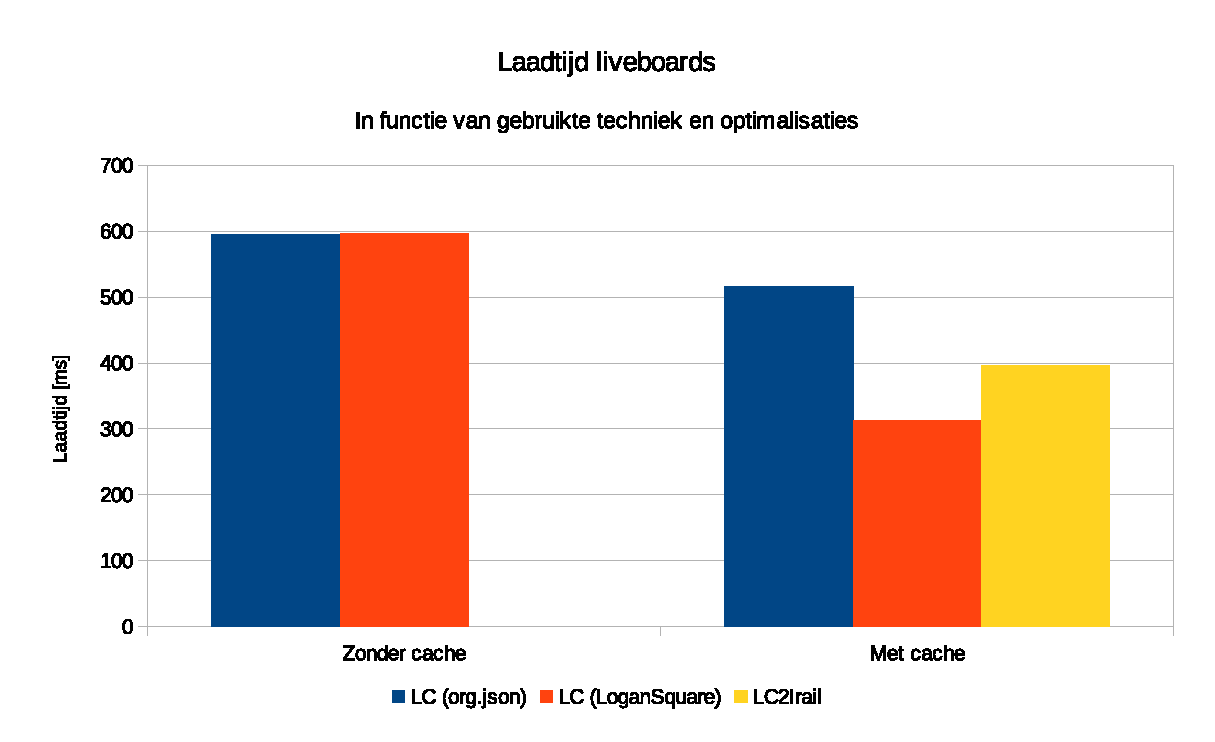
\includegraphics[width=0.80\textwidth]{Optimalisaties_liveboards.eps}
		\caption[Gemeten laadtijd liveboards]{De gemiddelde gemeten laadtijd voor liveboards gebruikmakend van een HTC 10 voor 262 opzoekingen gebaseerd op de iRail logs. }
	\label{fig:liveboardlabtest}
\end{figure}
%\begin{table}[h]
%	\begin{tabular}{| c | c | c | c | c | c |}
%		\hline
%		Variant & parser & cache & minimaal (ms) & gemiddelde (ms) & maximaal (ms)\\
%		\hline
%		LC op toestel & org.json & nee & 302 &  595 &  3471 \\
%		LC op toestel & org.json & ja & 409 &  516  &  3599 \\
%		LC op toestel & LoganSquare & nee & 392 & 597 & 2027 \\
%		LC op toestel & LoganSquare & ja  & 166 & 313 & 3428 \\
%		
%		LC op server &&&  232 & 397 &  1421\\
%		\hline
%	\end{tabular}
%	\caption[Gemeten laadtijd liveboards]{De gemeten laadtijd voor het eerste resultaat liveboards gebruikmakend van een HTC 10 voor 262 opzoekingen gebaseerd op de iRail logs. }
%	\label{tab:liveboardlabtest}
%\end{table}

Zoals eerder vermeld vergelijken we eerst kort verschillende implementaties van Linked Connections. In grafiek \ref{fig:liveboardlabtest} zijn de gemiddelde resultaten zichtbaar van een benchmark waarbij 262 stations opgezocht werden, ongeveer 5\% van de opzoekingen door gebruikers op 2 mei 2018. Telkens is de minimale, gemiddelde en maximale responstijd gemeten. Dit zowel gebruikmakend van de standaard (\foreign{org.json}) JSON parser en gebruikmakend van de \foreign{LoganSquare} parser. Ook werd de test herhaald met cache in- en uitgeschakeld, om zo het effect hiervan te meten. Tot slot werd dezelfde test herhaald gebruikmakend van data afkomstig van de LC2Irail web applicatie om een vergelijking tussen de twee methodes te kunnen maken. Deze cijfers geven slechts een indicatie van de snelheid - een volledige en diepgaande statistische analyse van de performantieverschillen tussen verschillende implementaties van dezelfde techniek valt wegens tijdsgebrek buiten het bereik van deze masterproef.

In deze cijfers is invloed van de cache duidelijk merkbaar. We zien wel een duidelijk verschil tussen de JSON parsers: terwijl bij gebruik van de \foreign{LoganSquare} parser de gemiddelde laadtijd bijna halveert, terwijl het effect van de cache bij het gebruik van de \foreign{org.json} parser veel kleiner is. Wanneer de cache uitgeschakeld is is het verschil tussen de parsers verwaarloosbaar. Dit is mogelijk te verklaren door het feit dat voor het tonen van vertrekken of aankomsten relatief weinig data nodig is: in de meeste gevallen volstaat een enkele Linked Connections pagina.

Om een exact beeld te vormen van de prestaties, zoeken we een duizendtal liveboards op. Hiervoor kiezen we elke vijfde opzoeking uit de iRail logs. Voor elk liveboard worden twintig resultaten geladen. De resultaten hiervan zijn zichtbaar in grafieken \ref{fig:liveboardsDiefBest}, \ref{fig:liveboardsDiefAvg} en \ref{fig:liveboardsDiefSlechtst}, respectievelijk voor het tiende, vijftigste en negentigste percentiel. Uit deze grafieken kunnen we duidelijke trends zien:

\begin{figure}[h]
	\centering
	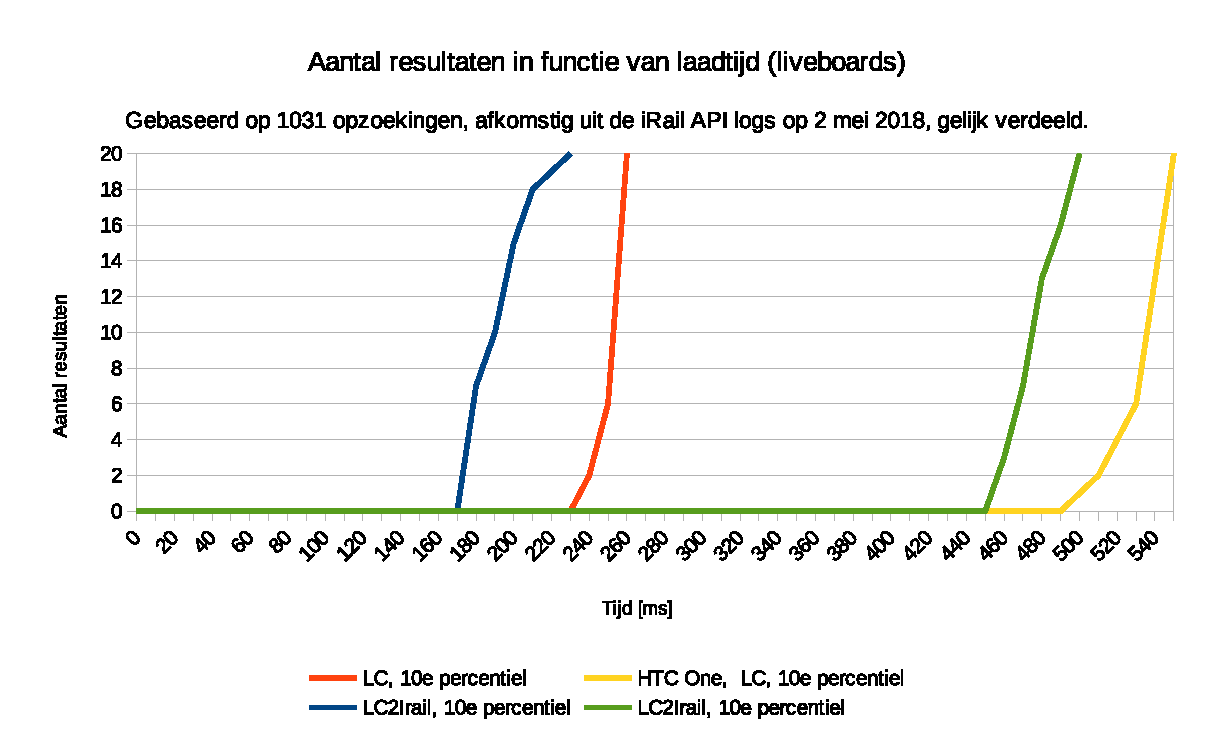
\includegraphics[width=1.00\textwidth]{dief_liveboards_best.eps}
	\caption[Aantal resultaten liveboards in functie van de tijd]{Het aantal resultaten in functie van de verlopen tijd.}
	\label{fig:liveboardsDiefBest}
\end{figure}

\begin{figure}[h]
	\centering
	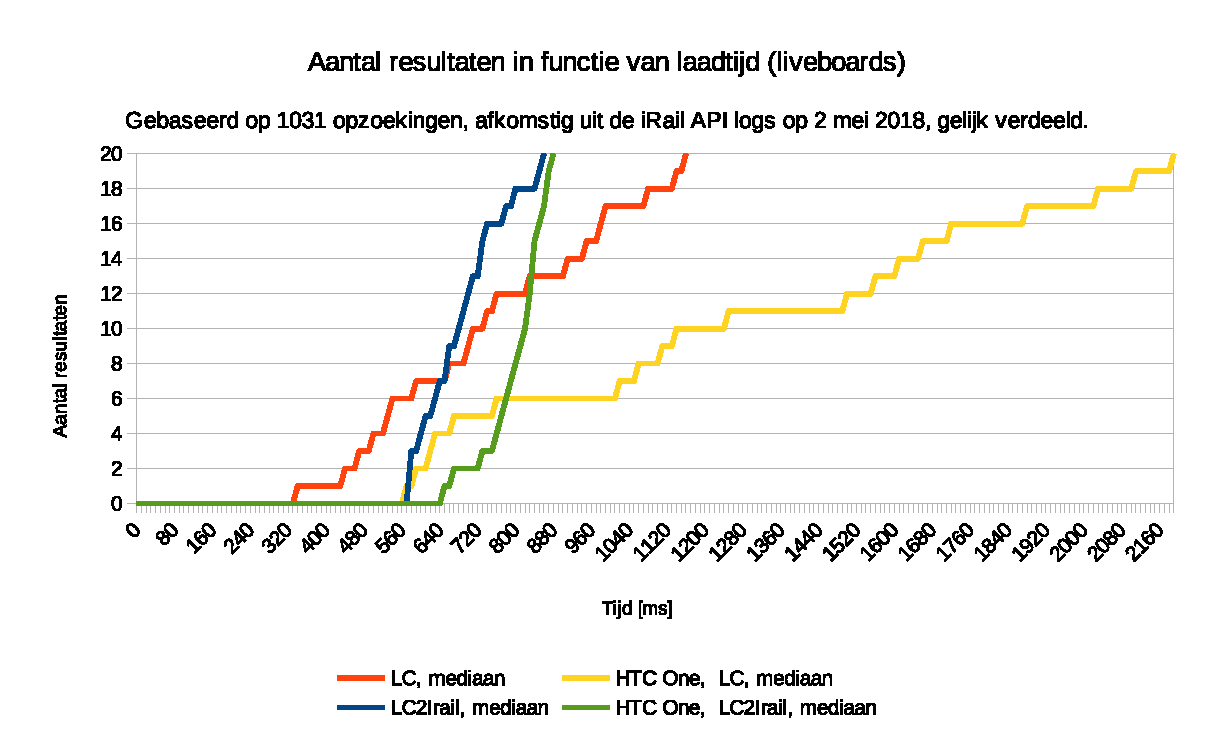
\includegraphics[width=1.00\textwidth]{dief_liveboards_gemiddeld.eps}
	\caption[Aantal resultaten liveboards in functie van de tijd]{Het aantal resultaten in functie van de verlopen tijd.}
	\label{fig:liveboardsDiefAvg}
\end{figure}

\begin{figure}[h]
	\centering
	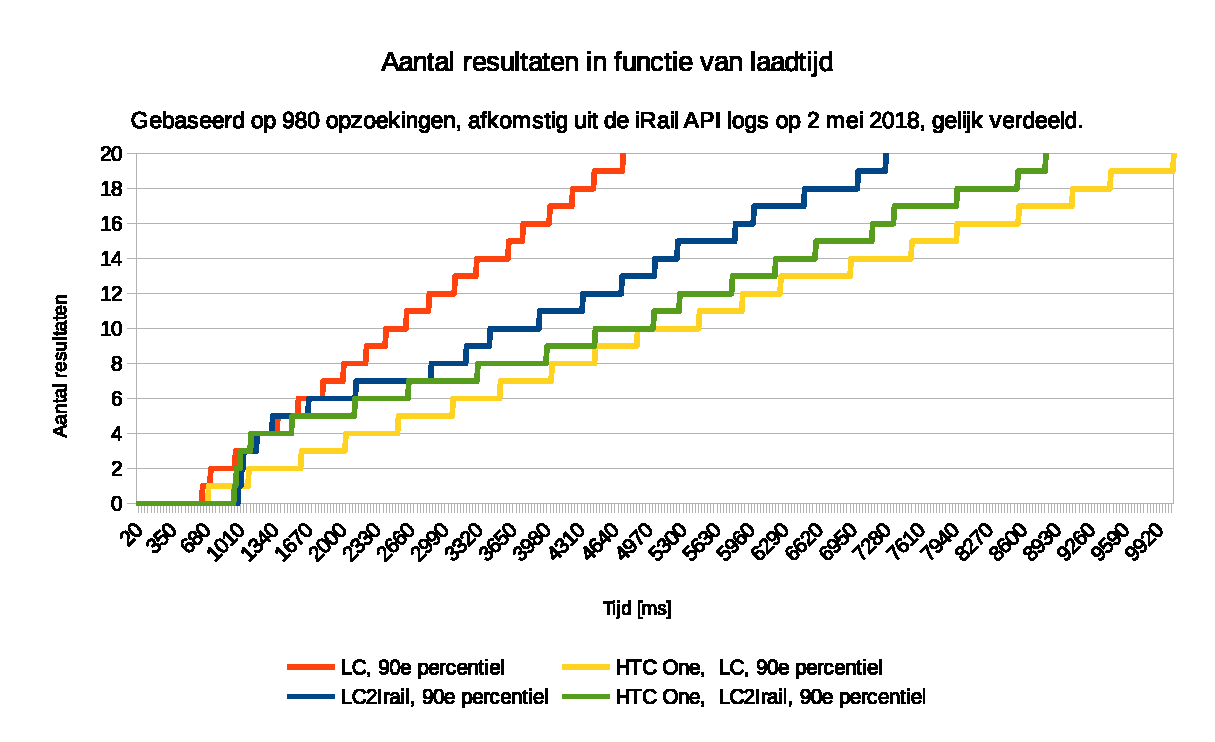
\includegraphics[width=1.00\textwidth]{dief_liveboards_slechtst.eps}
	\caption[Aantal resultaten liveboards in functie van de tijd]{Het aantal resultaten in functie van de verlopen tijd.}
	\label{fig:liveboardsDiefSlechtst}
\end{figure}


\begin{itemize}
    \item In de snelste gevallen is de serverimplementatie sneller. Hiervoor kunnen we verschillende oorzaken aanwijzen: 
	\begin{itemize}
		\item De serverimplementatie kan resultaten op een specifieke vraag cachen, terwijl de lokale implementatie deze steeds zal herberekenen vanaf Linked Connections pagina's. Voor veel voorkomende zoekopdrachten, zoals populaire stations, kan de server ook Linked Connections pagina's cachen.
		\item De serverimplementatie hoeft minder data te versturen. Ook het parsen van het antwoord gaat sneller, gezien slechts een kleine hoeveelheid data verwerkt moet worden en er verder geen berekeningen moeten gebeuren.
	\end{itemize}

	\item Terwijl in de snelste gevallen de serverimplementatie sneller is, is dit verschil beperkt tot ongeveer 60 milliseconden voor het eerste resultaat. Dit ligt zeer kort bij een verschil van 10\%, wat in deze ordegrootte moeilijk onderscheidbaar is voor gebruikers \citep{miller68}. %TODO CITE Weber-Fechner Law
	
	\item Wanneer we naar de mediane performantie kijken, is Linked Connections duidelijk sneller voor de eerste resultaten. Dit snelheidsverschil is aanzienlijk, en hoogstwaarschijnlijk vooral te wijten aan het feit dat Linked Connections volledige ondersteuning biedt voor incrementele resultaten, waarbij de server meestal meerdere pagina's zal overlopen voor een  antwoord gegeven wordt. Dit is te zien aan de steile curves voor LC2Irail, waar de curves voor LC gekenmerkt worden door een minder sterke stijging. 
	
	Anderzijds is er bij Linked Connections sprake van een \foreign{overhead} door het laden van te veel data. Voor stations met weinig vertrekken, of tijdens piekuren, kan het hierdoor meer moeite kosten om Linked Connections te verwerken. We vermoeden dat dit contrast met de korte, informatiedichte antwoorden van de RPC API zorgt voor het trager laden van resultaten. We zien dat hoe sneller het toestel, hoe langer Linked Connections het snelst blijft. Dit bevestigt de hypothese dat het verwerken van Linked Connections pagina's aan de oorzaak ligt. Ook blijft het verschil tussen Linked Connections en LC2Irail beperkt op de HTC 10, terwijl dit verschil aanzienlijk oploopt op de tragere HTC One.
	
	\item In alle gevallen is er een sterke gelijkenis tussen de curves voor LC2Irail op het HTC 10 toestel en het HTC One toestel. Deze zijn enkel een relatief kleine afstand in tijd verschoven, wat verklaart kan worden door de lage belasting voor het mobiele toestel wanneer een RPC API gebruikt wordt.

	\item Het verschil in laadtijd tussen Linked Connections op de twee toestellen loopt lineair op met de benodigde laadtijd om resultaten te laden. Zo zien we dat in het slechtste geval dubbel zoveel tijd benodigd is op de HTC One in vergelijking met de HTC 10. Dit is een sterke indicatie dat de performantie van Linked Connections afhankelijk is van het gebruikte toestel.
\end{itemize}

\begin{figure}[h]
	\centering
	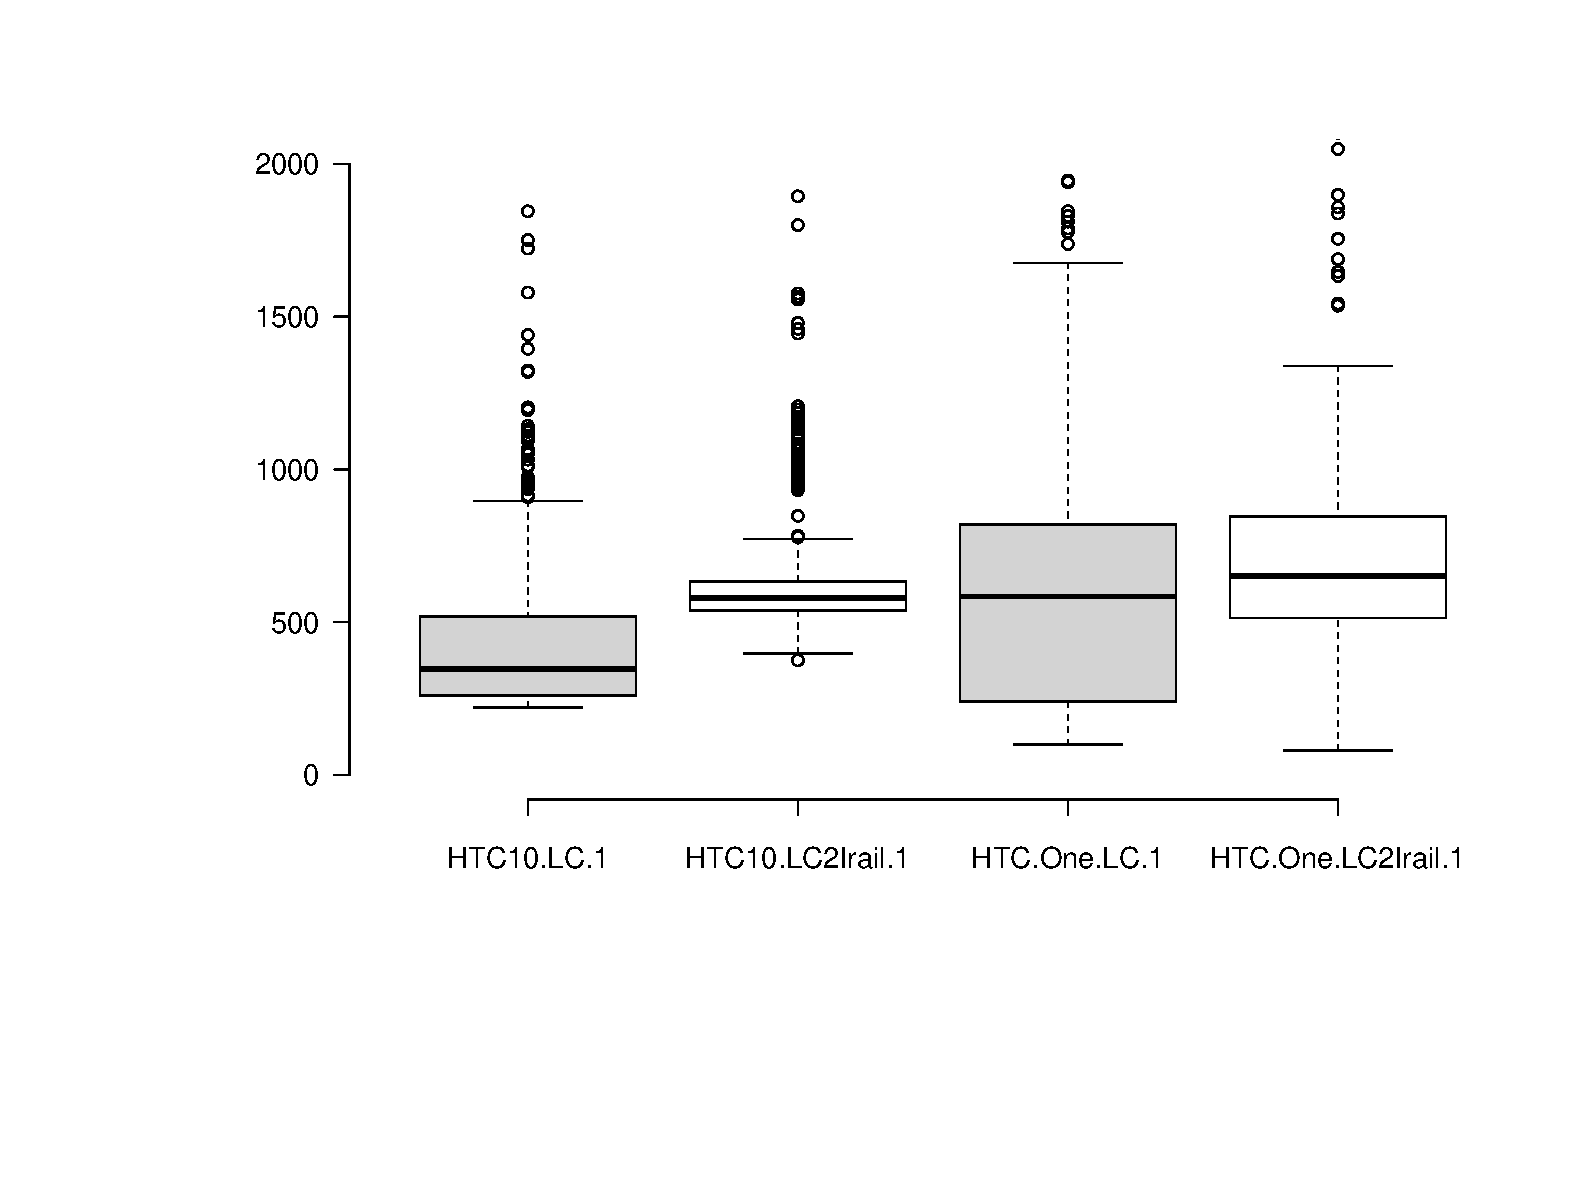
\includegraphics[width=1.00\textwidth]{boxplot_liveboards_1.eps}
	\caption[Laadtijd eerste resultaat liveboard in functie van toestel en technologie]{Laadtijd eerste resultaat liveboard in functie van toestel en technologie.}
	\label{fig:liveboardsBoxplot1}
\end{figure}

\begin{figure}[h]
	\centering
	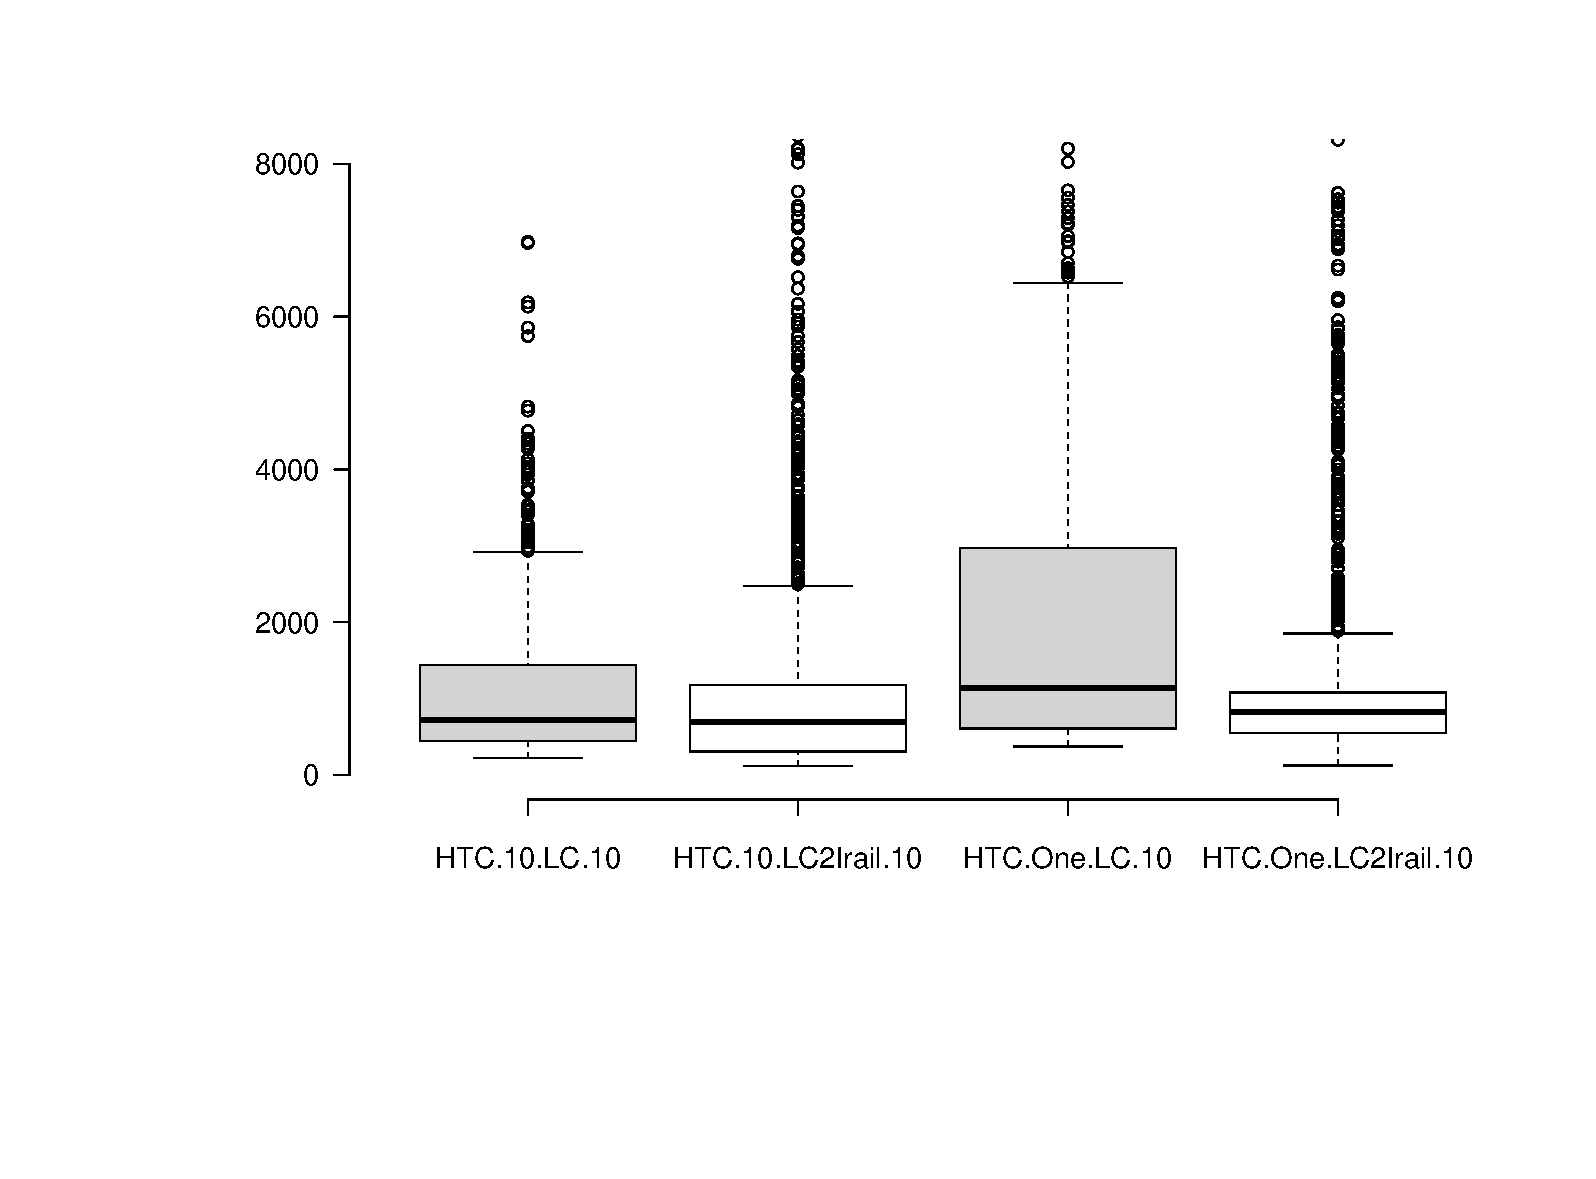
\includegraphics[width=1.00\textwidth]{boxplot_liveboards_10.eps}
	\caption[Laadtijd tiende resultaat liveboard in functie van toestel en technologie]{Laadtijd tiende resultaat liveboard in functie van toestel en technologie.}
	\label{fig:liveboardsBoxplot10}
\end{figure}

Wanneer we nu naar de spreiding van de laadtijden kijken, zichtbaar in figuur \ref{fig:liveboardsBoxplot1} voor het eerste resultaat en figuur \ref{fig:liveboardsBoxplot10} voor het tiende resultaat, zien we ook hier duidelijke verschillen tussen de verschillende methodes. Telkens levert LC2Irail een dichtere verdeling op dan LC, waarbij Linked Connections enkel sneller is voor het eerste resultaat op de HTC 10. Voor het eerste resultaat op de HTC One, en het tiende resultaat op de HTC 10, zijn beide implementaties volgens de wet van Weber-Fechner niet te onderscheiden op de mediaan.

In deze grafieken zijn ook de verschillen tussen toestellen enorm interessant. Zo zien we dat bij gebruik van een RPC API de mediaan van de laadtijd ongeveer gelijk is tussen verschillende toestellen, en de interkwartielafstand relatief klein is, wat op een kleine spreiding en dus consistente resultaten per toestel duidt. De mediaan voor beide toestellen ligt respectievelijk op 578 en 650 milliseconden voor het eerste resultaat. Volgens de wet van Weber-Fechner is dit onmerkbaar voor gebruikers. Ook het eerste kwartiel ligt kort genoeg bij elkaar om niet merkbaar te zijn. Ondanks dat we boven de mediaan zien dat opzoekingen via LC2Irail op de HTC One meer tijd vergen, is onder de mediaan voor gebruikers geen verschil merkbaar. Deze zeer consistente ervaring over toestellen is zeer wenselijk voor routeplanning applicatie. Voor het tiende resultaat neemt het verschil tussen de toestellen toe, waarbij gebruikers een verschil zullen merken tussen de LC2Irail implementatie op verschillende toestellen.

Bij gebruik van Linked Connections zien we duidelijke verschillen tussen de mediaan van de laadtijd bij verschillende toestellen. Ook de interkwartielafstand varieert tussen toestellen: zo is een ouder toestel niet enkel trager, maar is ook de spreiding veel groter, en zijn de resultaten dus minder consistent op oudere (tragere) toestellen. Anderzijds is Linked Connections in de meeste gevallen wel duidelijk sneller dan LC2Irail op de HTC 10.

Een eigenaardigheid is dat de minima voor de HTC One telkens lager liggen. Dit wordt vermoedelijk veroorzaakt door verschillende Android versies, met een verschillende aanpak op vlak van asynchrone scheduling.

\subsection{Ervaringen}
Wanneer we nu naar de ervaringen van gebruikers gaan kijken, stemmen deze ongeveer overeen met wat we zouden verwachten na evaluatie van de metingen.

Zoals we in figuren \ref{fig:liveboardsBoxplot1} en \ref{fig:liveboardsBoxplot10} konden zien blijkt uit testen dat de performantie van LC2Irail consistenter is, zowel in de vorm van een kleinere spreiding van de resultaten op eenzelfde toestel, als in de vorm van kleinere verschillen tussen toestellen. Ook bij de gebruikerservaring zien we dit terugkomen. Wanneer de ervaren snelheid wordt uitgezet in een boxplot per techniek, zichtbaar in figuur \ref{fig:liveboardsUx}, zien we net als bij de testen dat voor LC2Irail een heel consistente beoordeling wordt gegeven, terwijl deze voor Linked Connections veel meer uitgespreid, én iets lager ligt.

\begin{figure}[h]
	\centering
	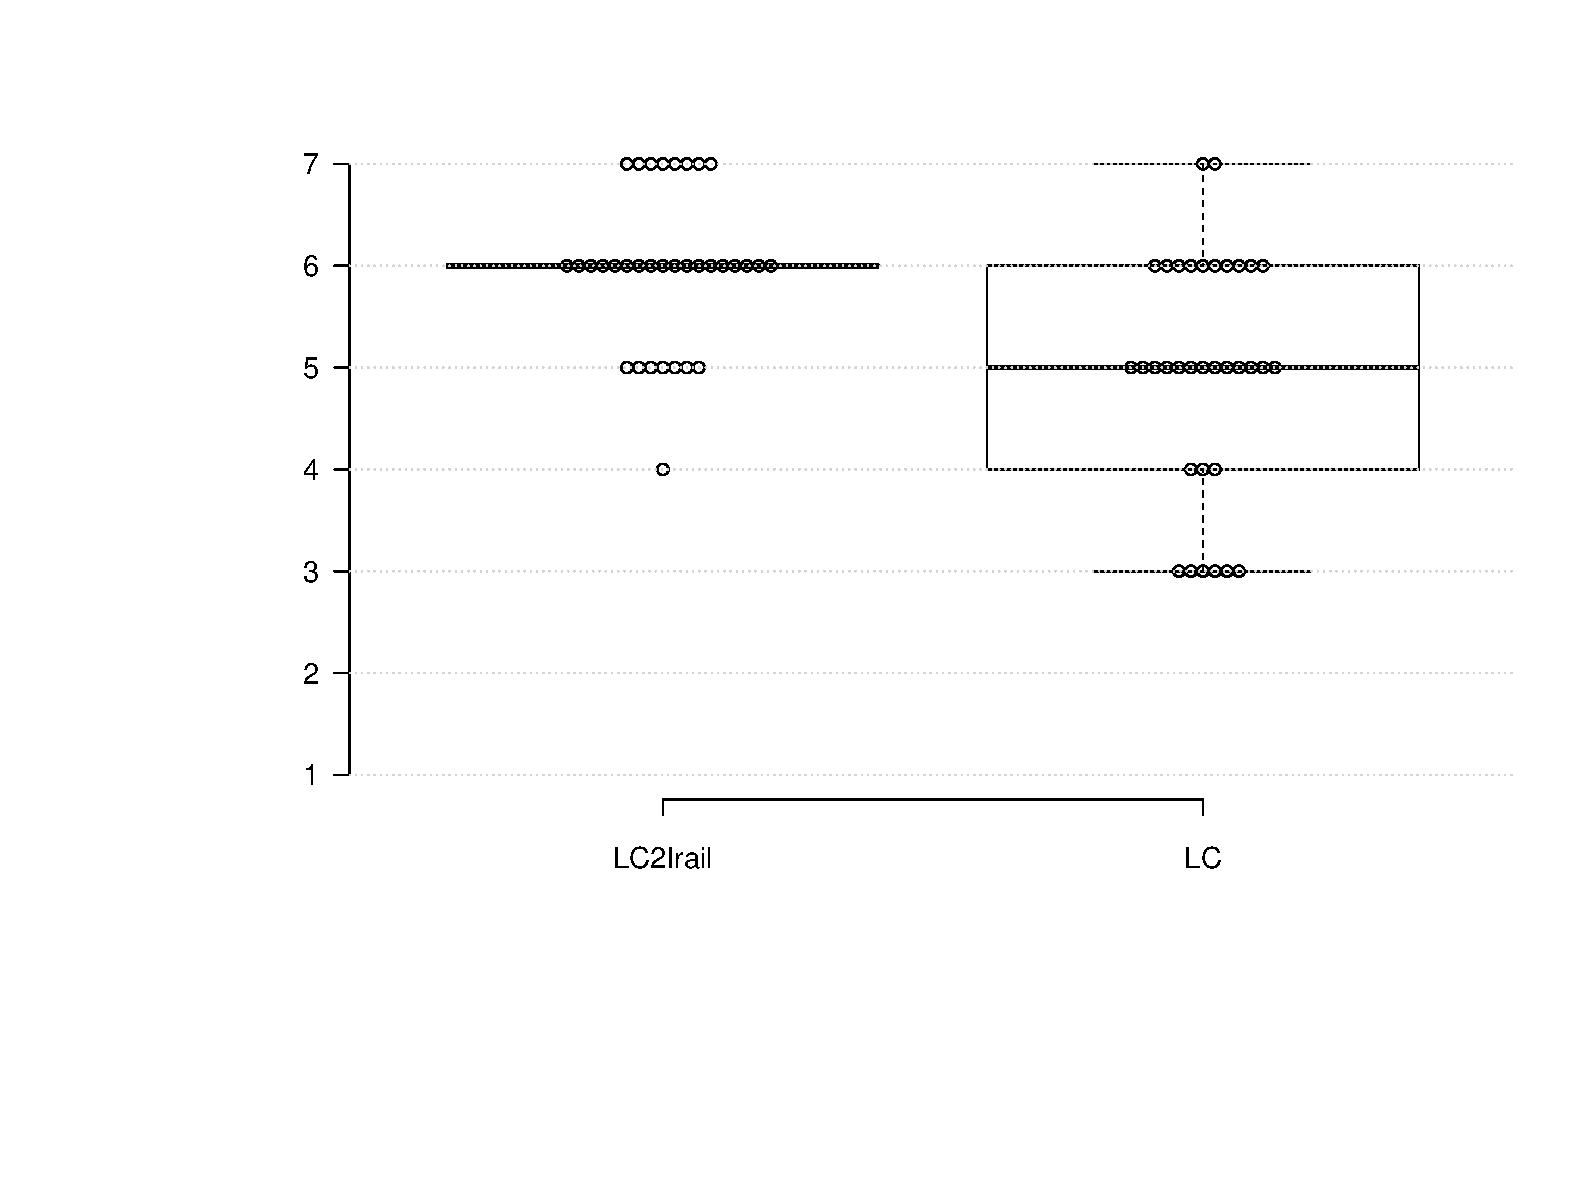
\includegraphics[width=0.80\textwidth]{boxplot_liveboards_ux.eps}
	\caption[Ervaren snelheid van liveboards]{De ervaren snelheid op een schaal 1-7 van vertrekken en aankomsten voor LC2Irail en Linked Connections, gebaseerd op 17 user tests.}
	\label{fig:liveboardsUx}
\end{figure}

Hoewel 12 van de 17 testpersonen Linked Connections als redelijk tot extreem snel ervaart, zijn er slechts twee personen die Linked Connections sneller ervaren dan LC2Irail. De ervaringen en uiteindelijk keus op basis van snelheid is zichtbaar in figuur \ref{fig:alluvialUserChoicesLiveboards}. Het is duidelijk zichtbaar dat de ervaringen voor Linked Connections veel gemengder zijn dan de ervaringen voor LC2Irail. Er zijn zowel mensen die Linked Connections sneller, even snel of trager ervaren. 

\begin{figure}[ht]
	\centering
	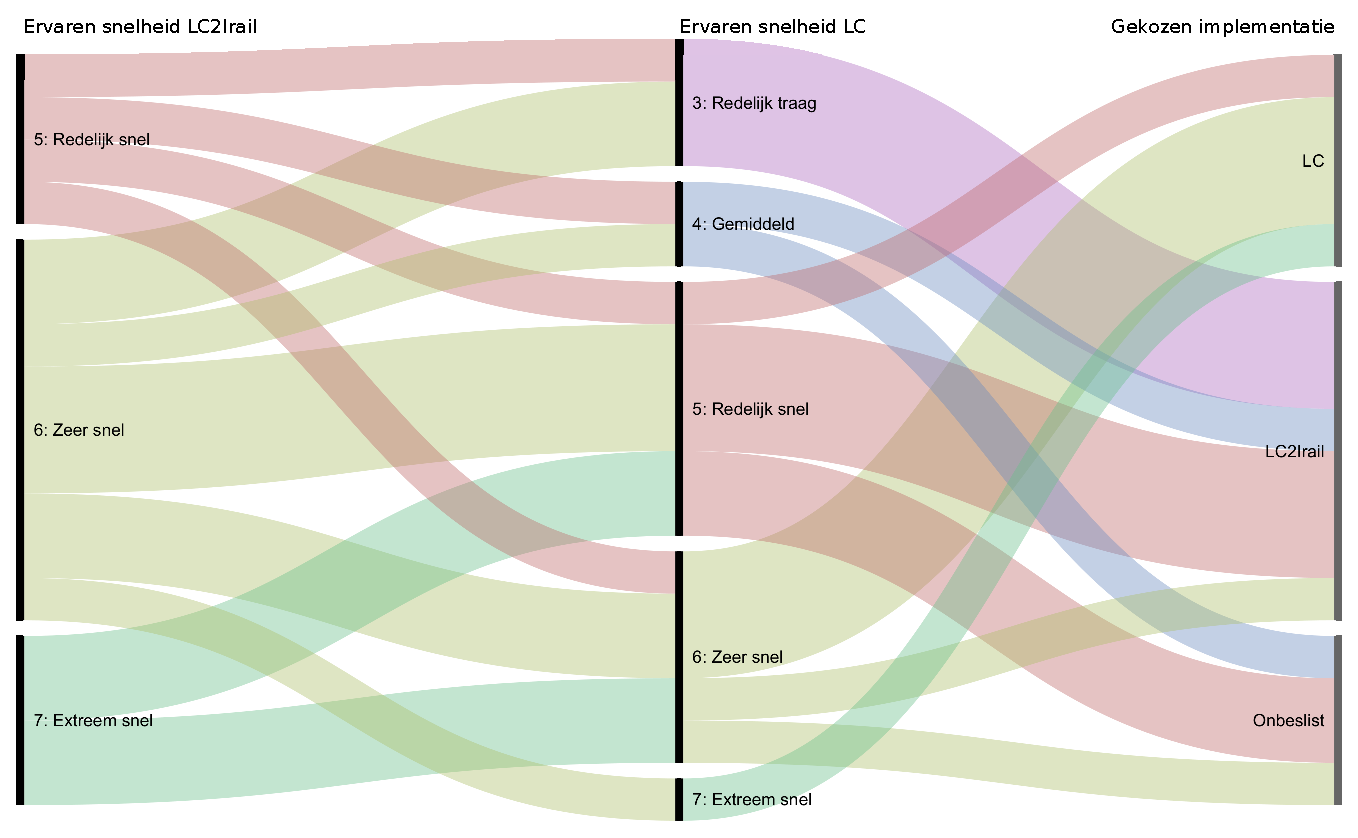
\includegraphics[width=1.00\textwidth]{alluvial_user_choice_departures.eps}
	\caption[Door gebruikers gekozen implementatie voor liveboards]{Verbanden tussen de door gebruikers gekozen implementaties voor liveboards. }
	\label{fig:alluvialUserChoicesLiveboards}
\end{figure}

Alle testpersonen werden expliciet gevraagd welke implementatie ze als sneller ervoeren. Hierbij waren de antwoorden verdeeld: acht personen kozen de Linked Connections, vier personen hadden geen mening, en vijf personen kozen LC2Irail variant. Het is moeilijk om hier onmiddelijk conclusies uit te trekken. Om deze reden zullen we in hoofdstuk \ref{chap:interpretatie} de resultaten algemener bespreken. Wel kunnen we zeggen dat gebruikerservaringen zeer gemengd zijn voor Linked Connections, en zal Linked Connections zoiezo niet voor de volledige populatie sneller zijn.

Wanneer we gaan kijken naar de verschillen tussen de JSON parsers, blijkt dat beide parsers ongeveer even goed presteren in de ogen van de testers. Respectievelijk 5 op 7 en 7 op 10 testers zijn neutraal of tevreden, en bij beide varianten is er telkens een tester neutraal. Deze vergelijking is echter slechts een indicatie, en is door te kleine steekproeven ongeschikt om te veralgemenen naar een grotere populatie.

Wanneer echter gekeken wordt naar de gemeten prestatieverschillen tussen beide JSON parsers tijdens de usertests, zien we een duidelijk verschil, waarbij het 90e percentiel van de laadtijd onder de LoganSquare parser lager ligt dan de mediane laadtijd van de org.json parser. Dit verschil lijkt echter geen invloed te hebben op de ervaringen van gebruikers, vermoedelijk omdat men beide reeds als performant genoeg ervaart. % TODO: Hoe groot procentueel verschil?

\begin{figure}[ht]
	\centering
	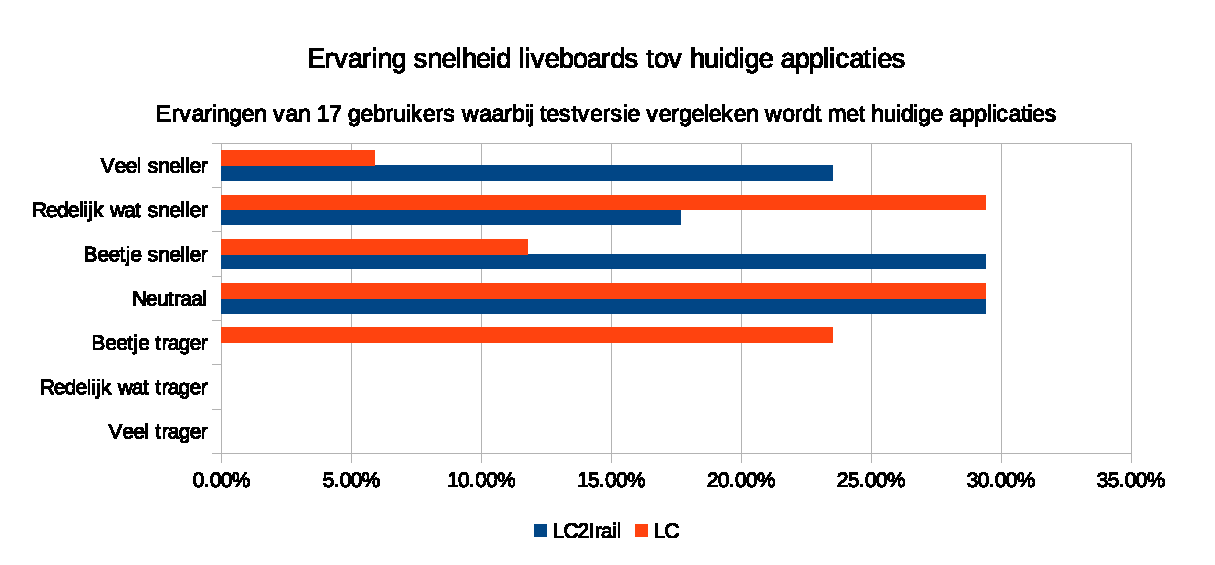
\includegraphics[width=1.00\textwidth]{userdata_liveboards_currentapp.eps}
	\caption[Door gebruikers ervaren snelheid liveboards tov huidige apps]{De door 17 gebruikers ervaren snelheid liveboards ten opzichte huidige apps }
	\label{fig:relativePerceptionLiveboards}
\end{figure}

Als tot slot gevraagd wordt om de snelheid te vergelijken met de applicatie die de gebruiker op dit moment gebruikt, zichtbaar in figuur \ref{fig:relativePerceptionLiveboards} , komen beide apps er goed uit. LC2Irail scoort hier zeer goed, en ondanks dat Linked Connections iets minder goed scoort dan LC2Irail, geven slechts 2 gebruikers aan Linked Connections trager te ervaren dan hun huidige applicatie.

\section{Routes}

\subsection{Metingen}
\begin{figure}[h]
	\centering
	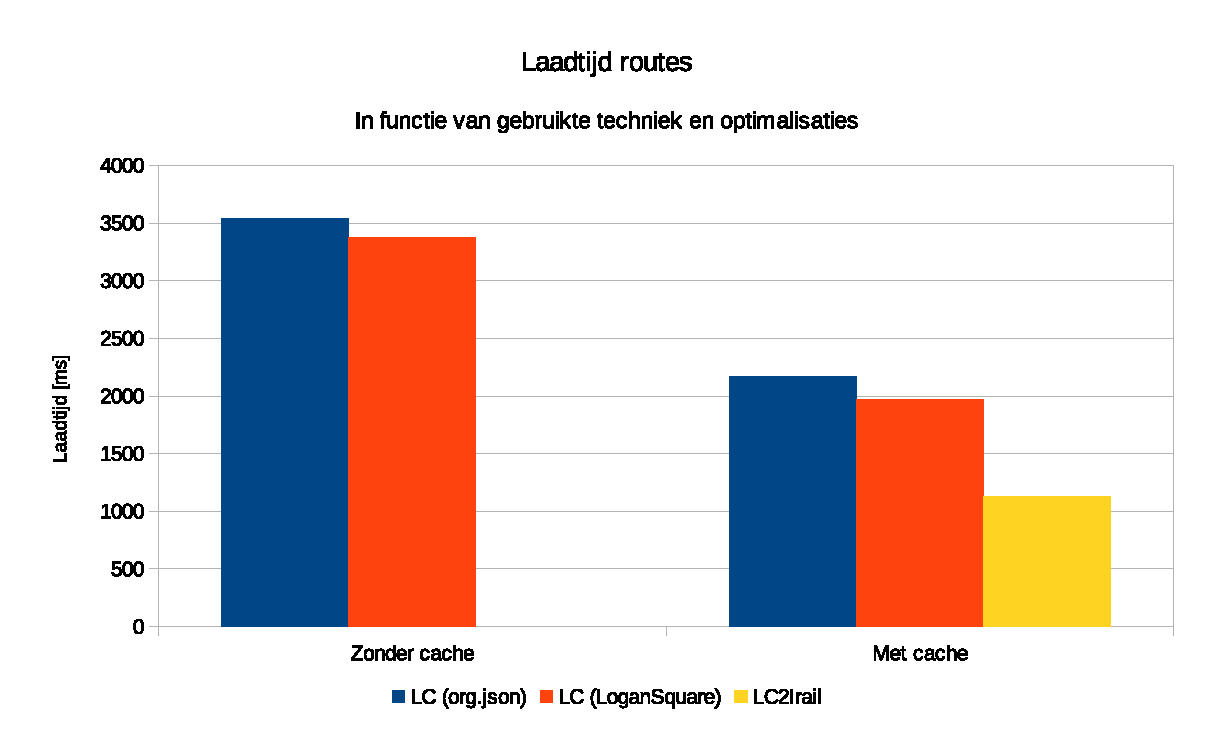
\includegraphics[width=0.80\textwidth]{Optimalisaties_routes.eps}
	\caption[Gemeten laadtijd routes]{De gemiddelde gemeten laadtijd voor routes gebruikmakend van een HTC 10 voor 779 opzoekingen gebaseerd op de iRail logs.}
	\label{fig:routelabtest}
\end{figure}
%\begin{table}[h]
%	\begin{tabular}{| c | c | c | c | c | c |}
%		\hline
%		Variant & parser & cache & minimaal (ms) & gemiddelde (ms) & maximaal (ms)\\
%		\hline
%		LC op toestel & org.json & nee & 401 & 3539 & 8531\\
%		LC op toestel & org.json & ja & 221 & 2172 & 6960 \\
%		LC op toestel & LoganSquare & nee &  386 & 3374 & 7554 \\
%		LC op toestel & LoganSquare & ja  & 233 & 1973 & 7640 \\
%		
%		LC op server &&&  27 & 1126 & 3374\\
%		\hline
%	\end{tabular}
%	\caption[Gemeten laadtijd routes]{De gemeten laadtijd voor routes gebruikmakend van een HTC 10 voor 779 opzoekingen gebaseerd op de iRail logs.}
%	\label{tab:routelabtest}
%\end{table}

Ook voor routes zullen we eerst kort de relatieve prestaties van verschillende implementaties bespreken. In grafiek \ref{fig:routelabtest} zijn de gemiddelde resultaten zichtbaar van een benchmark waarbij 779 routes opgezocht werden, ongeveer 5\% van de opzoekingen door gebruikers op 2 mei 2018. Telkens is de minimale, gemiddelde en maximale responstijd gemeten. Dit zowel gebruikmakend van de standaard JSON parser (\foreign{org.json}) en gebruikmakend van de \foreign{LoganSquare} parser. Ook werd de test herhaald met cache in- en uitgeschakeld, om zo het effect hiervan te meten. Tot slot werd dezelfde test herhaald gebruikmakend van data afkomstig van de LC2Irail web applicatie om een vergelijking tussen de twee methodes te kunnen maken. Deze cijfers geven slechts een indicatie van de snelheid - een volledige en diepgaande statistische analyse van de performantieverschillen tussen verschillende implementaties van dezelfde techniek valt wegens tijdsgebrek buiten het bereik van deze masterproef.

Net zoals bij liveboards is ook hier de invloed van de cache duidelijk merkbaar. Dit valt te verklaren door de grote hoeveelheden data die verwerkt moeten worden, waarbij het cruciaal is dat deze niet steeds opnieuw gedownload wordt. Vergeleken met dezelfde analyse voor Liveboards (figuur \ref{fig:liveboardlabtest}), zien we hier een minder groot verschil tussen de parsers. Dit komt mogelijk door de grotere impact van de verdere algoritmes, waardoor de invloed van parsing verkleint. Het algoritme om de data tot routes te verwerken is het zwaarst van de drie endpoints. %TODO: remove LC2Irail from graph

Om ook hier een exact beeld te vormen van de prestaties, maken we ook hier een duizendtal opzoekingen. Hiervoor kiezen we telkens de vijfde opzoeking uit de iRail logs. Voor elke route wordt gepoogd 10 resultaten geladen. De resultaten hiervan zijn zichtbaar in grafieken \ref{fig:routesDiefBest}, \ref{fig:routesDiefAvg} en \ref{fig:routesDiefSlechtst}, respectievelijk voor het tiende, vijftigste en negentigste percentiel.

\begin{figure}[h]
	\centering
	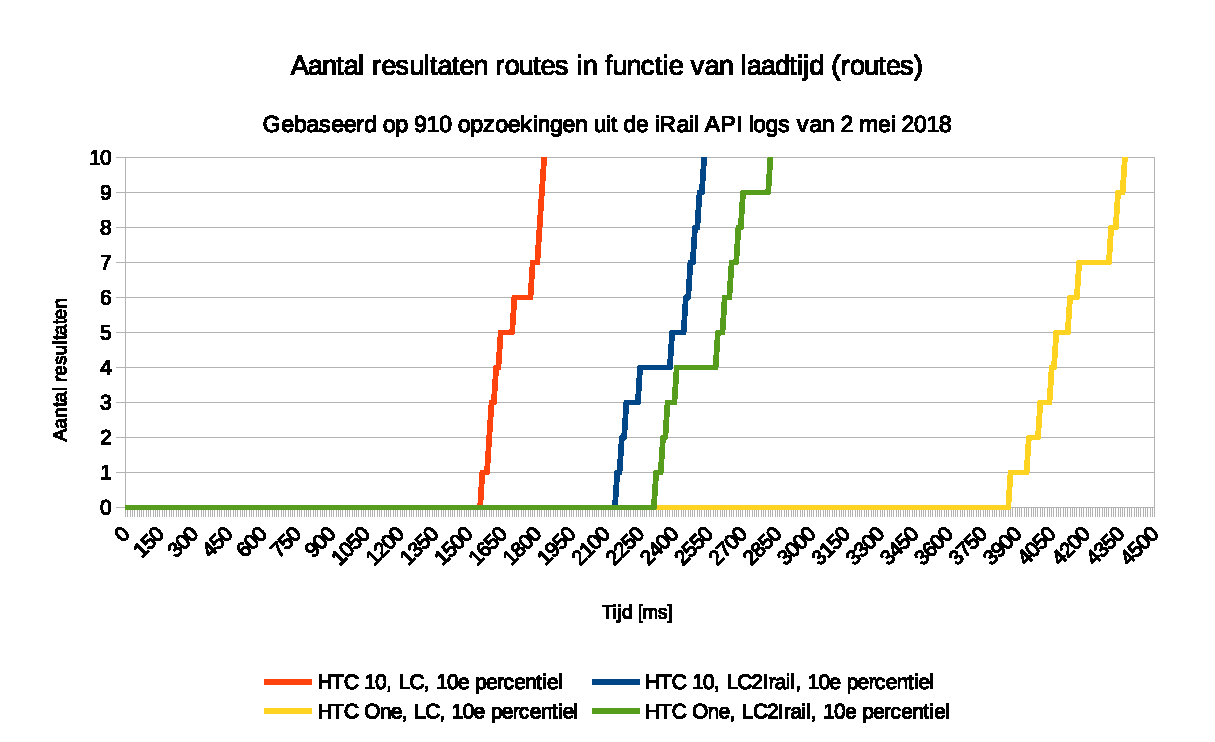
\includegraphics[width=1.00\textwidth]{dief_routes_best.eps}
	\caption[Aantal resultaten routes in functie van de tijd]{Het aantal resultaten in functie van de verlopen tijd.}
	\label{fig:routesDiefBest}
\end{figure}

\begin{figure}[h]
	\centering
	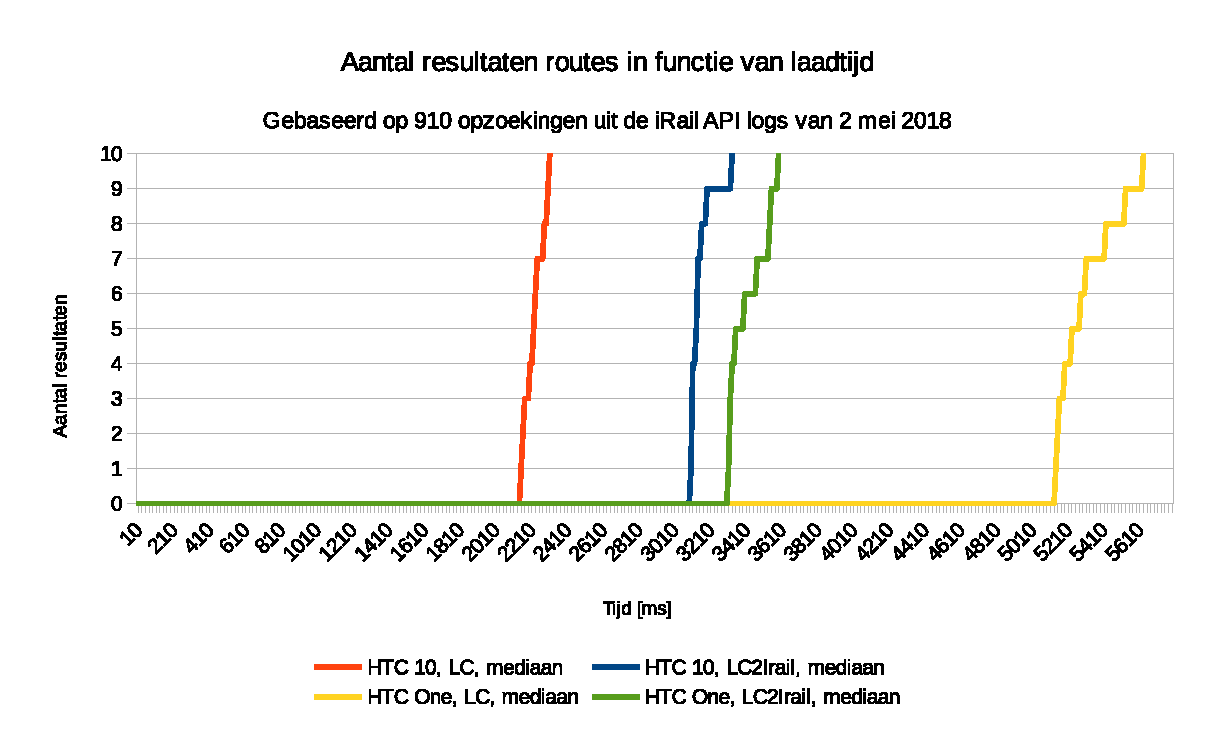
\includegraphics[width=1.00\textwidth]{dief_routes_gemiddeld.eps}
	\caption[Aantal resultaten routes in functie van de tijd]{Het aantal resultaten in functie van de verlopen tijd.}
	\label{fig:routesDiefAvg}
\end{figure}

\begin{figure}[h]
	\centering
	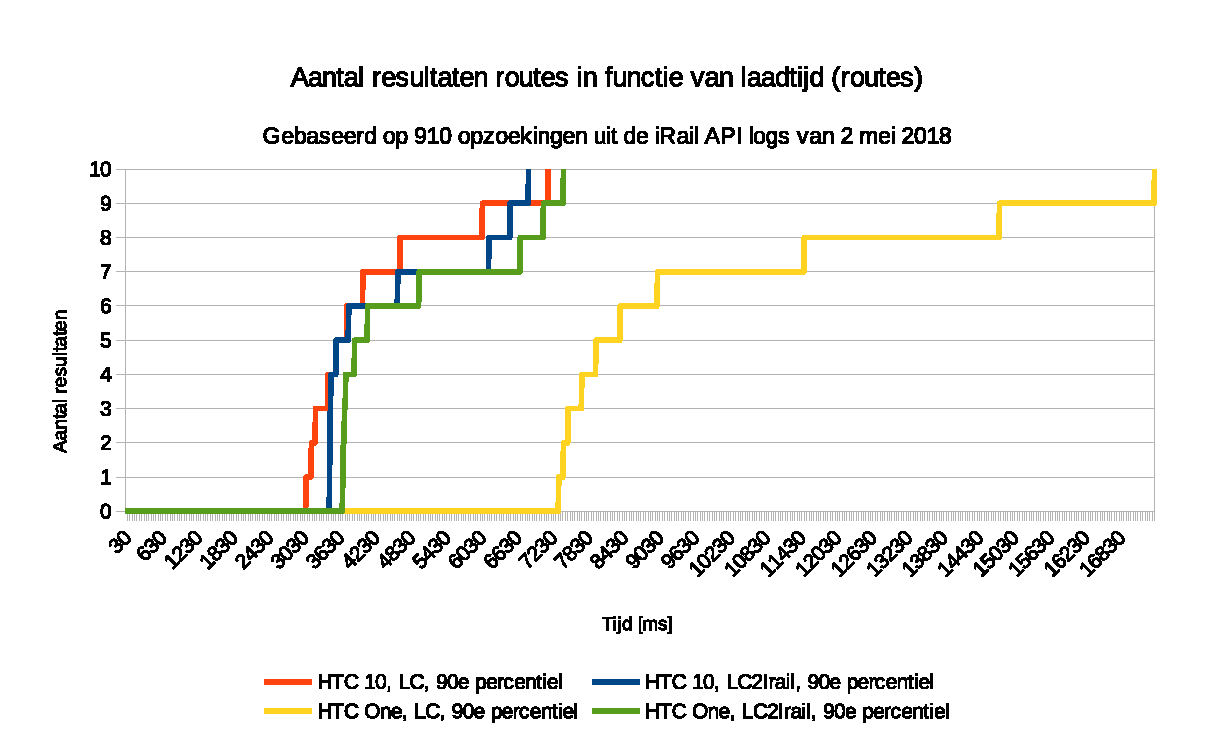
\includegraphics[width=1.00\textwidth]{dief_routes_slechtst.eps}
	\caption[Aantal resultaten routes in functie van de tijd]{Het aantal resultaten in functie van de verlopen tijd.}
	\label{fig:routesDiefSlechtst}
\end{figure}

Uit deze grafieken kunnen we opnieuw duidelijke conclusies trekken:
\begin{itemize}
	\item In alle grafieken en voor alle testen, hebben de curves een gelijkaardige vorm, waarbij er na een relatief lange wachttijd aan snel tempo resultaten geladen worden: in het geval van Linked Connections is voor de eerste opzoeking telkens een relatief grote hoeveelheid data nodig is, waarna slechts één of twee extra pagina's moeten opgehaald worden om het volgend resultaat te bepalen. In het geval van LC2Irail worden resultaten in grote blokken binnengehaald, waarbij vanaf de tweede opzoeking reeds veel data in cache zit. In het geval van LC2Irail worden resultaten ook onmiddellijk voor grote intervallen opgehaald, om zo het aantal verzoeken te beperken. 
	\item Terwijl op de HTC 10 Linked Connections in alle gevallen beter presteert dan LC2Irail, presteert Linked Connections slechter dan LC2Irail op de HTC One. 
	\item Opnieuw presteert LC2Irail op beide toestellen gelijkaardig, met slechts een kleine verschuiving in tijd tussen beide curves.
	\item Terwijl in het slechtste geval bijna alle varianten gelijk presteren, loopt Linked Connections op de HTC One enorm achter. Uit alle grafieken volgt dat hoe trager het toestel, hoe trager Linked Connections, terwijl LC2Irail ongeveer even goed blijft presteren. Bijgevolg kunnen we dus ook stellen, dat alle toestellen trager dan de HTC10 in het slechtste geval trager zullen presteren dan de HTC One.
	\item In alle gevallen laadt het eerste resultaat pas na anderhalve tot zeven seconden. Dit zijn zeer lange laadtijden, waarvan we verwachten dat ze de gebruikerservaring negatief gaan beïnvloeden.
\end{itemize}

Wanneer we nu specifiek naar de verdelingen kijken, gevisualiseerd door middel van de box plots in figuur \ref{fig:routesBoxplot1} en \ref{fig:routesBoxplot10}, zien we sterke verschillen, zowel tussen toestellen als implementaties. Net als bij liveboards zien we ook hier duidelijk hoe LC2Irail gelijke prestaties heeft op beide toestellen, met bijna identieke distributies. Dit in tegenstelling tot de prestaties van Linked Connections, die zeer sterk variëren per toestel. Op de HTC 10 zal voor al meer dan 75\% van de opzoekingen via Linked Connections het eerste resultaat geladen zijn op het moment dat LC2Irail op hetzelfde toestel minder dan 25\% van de verzoeken beantwoordt heeft. Op het HTC One toestel is dit echter omgekeerd, en nog extremer. 

Voor het tiende resultaat zijn deze verschillen tussen toestellen iets minder extreem, al zijn ze nog steeds zeer groot. Linked Connections blijft iets consistentere resultaten bieden op de HTC 10, terwijl de HTC One net minder consistente resultaten biedt dan LC2Irail. LC2Irail biedt ook voor het tiende resultaat exact dezelfde ervaring op beide toestellen, terwijl het verschil tussen de mediaan voor Linked Connections op beide toestellen niet acceptabel is en de gebruikerservaring duidelijk zal beïnvloeden.

\begin{figure}[h]
	\centering
	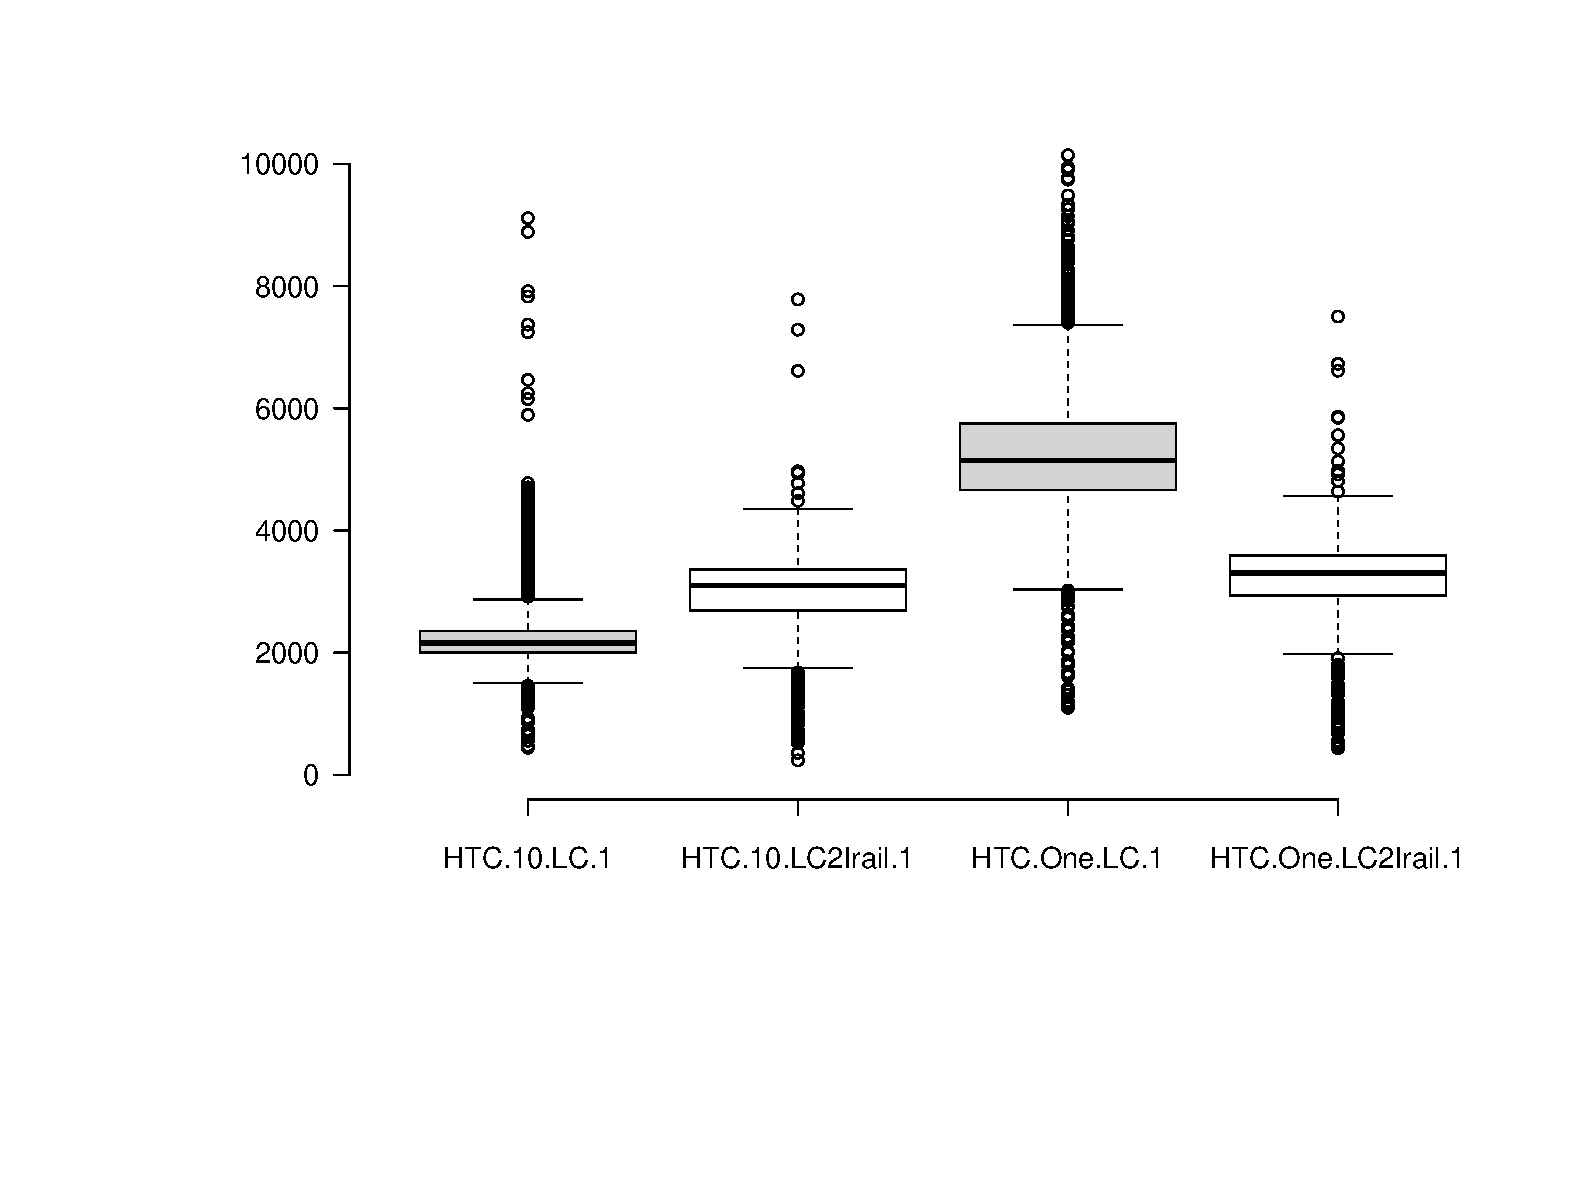
\includegraphics[width=0.80\textwidth]{boxplot_routes_1.eps}
	\caption[Laadtijd eerste resultaat route in functie van toestel en technologie]{Laadtijd eerste resultaat route in functie van toestel en technologie.}
	\label{fig:routesBoxplot1}
\end{figure}

\begin{figure}[h]
	\centering
	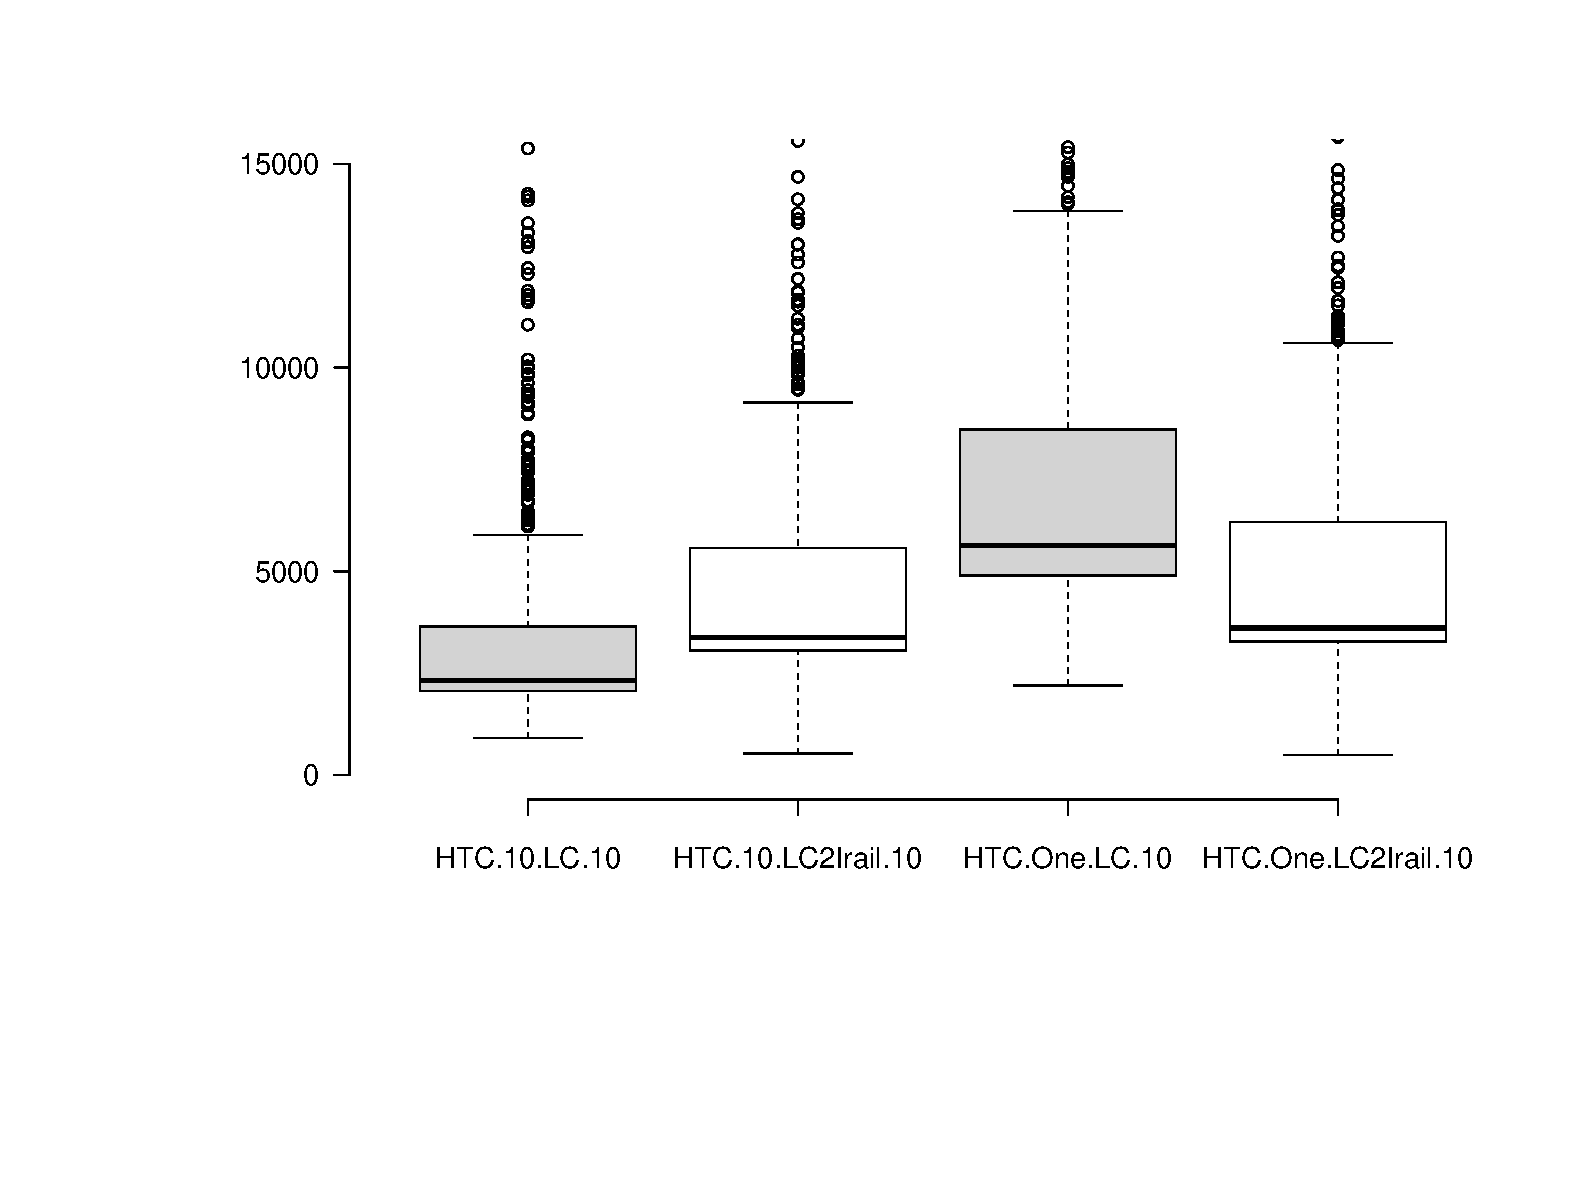
\includegraphics[width=0.80\textwidth]{boxplot_routes_10.eps}
	\caption[Laadtijd tiende resultaat route in functie van toestel en technologie]{Laadtijd tiende resultaat route in functie van toestel en technologie.}
	\label{fig:routesBoxplot10}
\end{figure}

\subsection{Ervaringen}

Op vlak van gebruikerservaring verwachten we dat gebruikers net zoals bij Liveboards de implementatie op basis van LC2Irail consistenter zullen beoordelen, en dat, afhankelijk van het door de tester gebruikte toestel, Linked Connections sneller, even snel of trager dan LC2Irail ervaren wordt.

\begin{figure}[h]
	\centering
	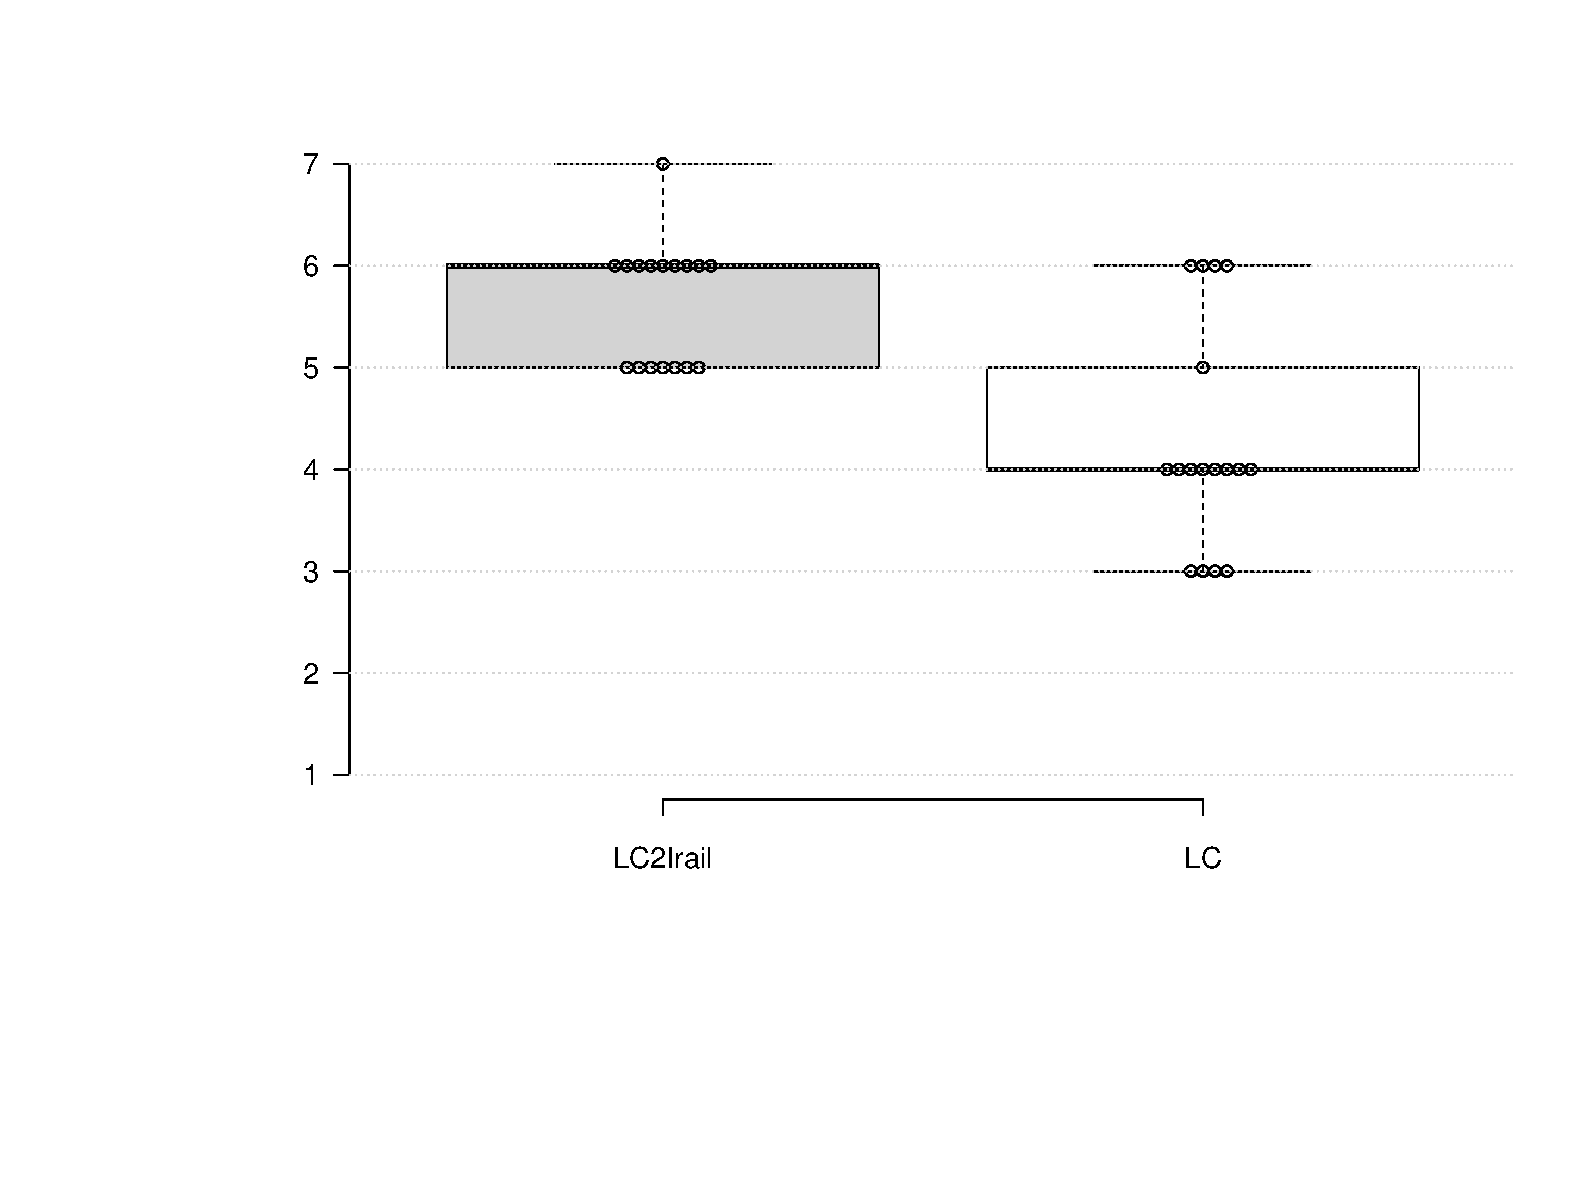
\includegraphics[width=0.80\textwidth]{boxplot_routes_ux.eps}
	\caption[Ervaren snelheid van routes]{De ervaren snelheid op een schaal 1-7 van routes voor LC2Irail en Linked Connections, gebaseerd op 17 user tests.}
	\label{fig:routesUx}
\end{figure}

Wanneer we nu de resultaten van user-testing vergelijken met de verwachtingen, blijken deze verwachtingen grotendeels in vervulling te gaan. In figuur \ref{fig:routesUx} is te zien dat de prestaties van LC2Irail iets consistenter goed beoordeeld worden, en LC2Irail een betere beoordeling krijgt dan Linked Connections. In vergelijking met liveboards (figuur \ref{fig:liveboardsUx}) zien we dat gebruikers bij routes iets minder verdeeld zijn over de prestaties van Linked Connections, al komt dit omdat er geen gebruikers voor de hoogste score kiezen. 

De consistentere beoordelingen voor Linked Connections zijn ook duidelijk wanneer we dieper ingaan op hoe eenzelfde gebruiker de snelheid van LC2Irail en Linked Connections ervaart, zichtbaar in figuur \ref{fig:alluvialUserChoicesRoutes}. Hoewel veel gebruikers Linked Connections als trager ervaren, is er ook een klein aantal gebruikers dat Linked Connections sneller ervaart. Het zijn deze personen die, wanneer expliciet gevraagd wordt om de snelste implementatie aan te duiden, voor Linked Connections kiezen. Dit duidelijk verband kon bij liveboards niet gelegd worden (figuur \ref{fig:alluvialUserChoicesLiveboards}), wat te wijten kan zijn aan een voor gebruikers slechts een klein, onduidelijk verschil was tussen de prestaties bij liveboards. Voor routes wordt het verschil veel duidelijker ervaren, en kiezen gebruikers dus consistenter met de door hun ervaren snelheden.

Opvallend is ook dat er een persoon is die Linked Connections als zeer snel bestempelt, en Linked Connections hiermee even snel of sneller dan LC2Irail ervaart. Echter kiest deze persoon toch voor LC2Irail wanneer een expliciete keuze gemaakt dient te worden. We kunnen stellen dat voor deze gebruiker het verschil niet merkbaar was. Aan de andere kant kiest iedereen die Linked Connections als traag of gemiddeld ervaart voor LC2Irail, op één gebruiker na die onbeslist is. Voor deze gebruikers moet Linked Connections nog sneller gemaakt worden alvorens het concurrentieel wordt.

\begin{figure}[ht]
	\centering
	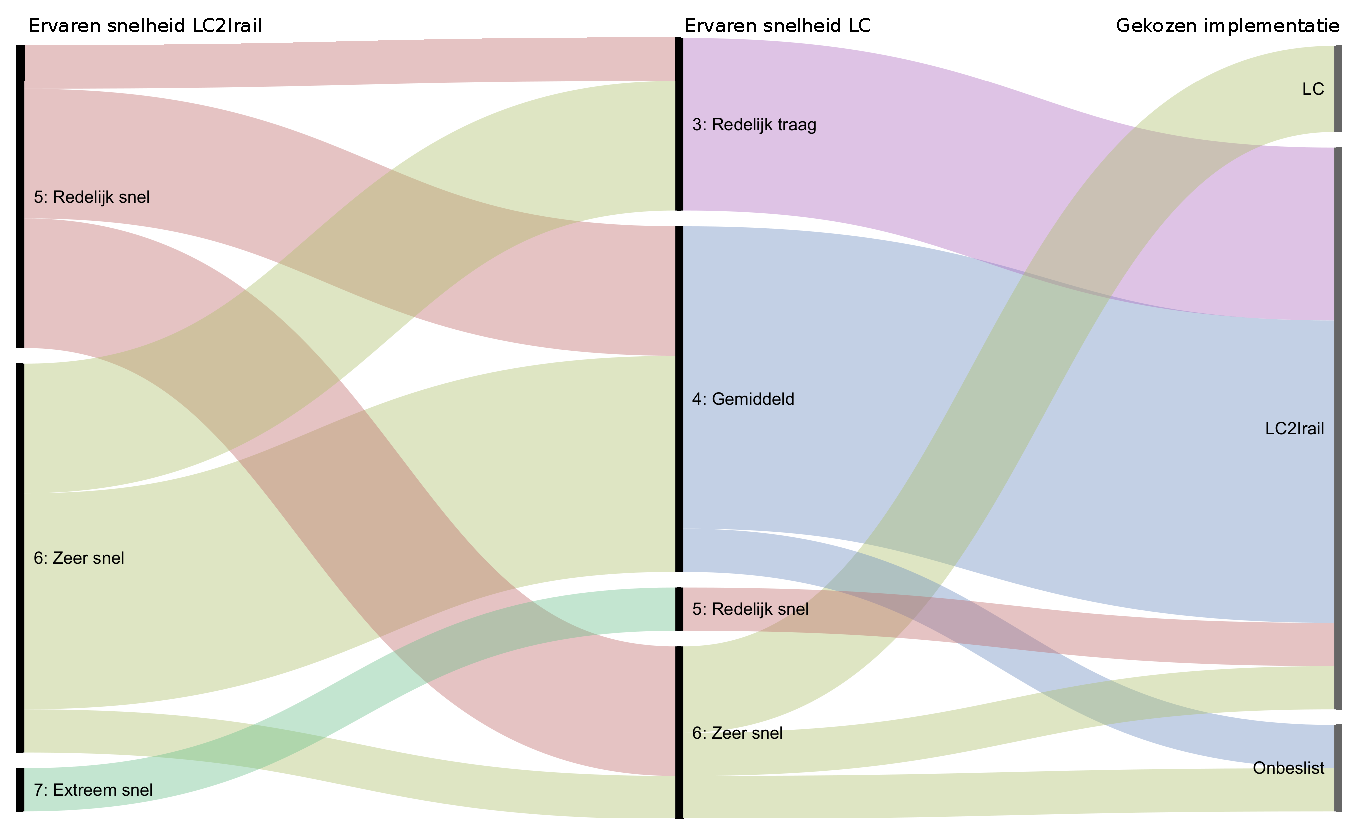
\includegraphics[width=1.00\textwidth]{alluvial_user_choice_routes.eps}
	\caption[Door gebruikers gekozen implementatie voor routes]{Verbanden tussen de door gebruikers gekozen implementaties voor routes. }
	\label{fig:alluvialUserChoicesRoutes}
\end{figure}

Wanneer we voor routes beide JSON parsers vergelijken, zien we dat voor de \foreign{LoganSquare} parser de proefpersonen een meer uitgesproken mening hadden: er waren zowel meer tevreden als ontevreden personen, terwijl bij de \foreign{org.json} parser veel mensen neutraal waren. Dit gaat echter in tegen een praktijktest waarbij enkele gebruikers achtereenvolgens een versie gebruikmakend van de \foreign{org.json} en \foreign{LoganSquare} parser voorgeschoteld kregen, gaven deze telkens aan de versie op basis van \foreign{LoganSquare} sneller te ervaren, zowel op goedkope als dure smartphones. Hieruit besluiten we dat de gebruikerstests, opgedeeld per parser, te kleine steekproeven zijn om een algemene conclusie te vormen over de invloed van de parsers.

\begin{figure}[ht]
	\centering
	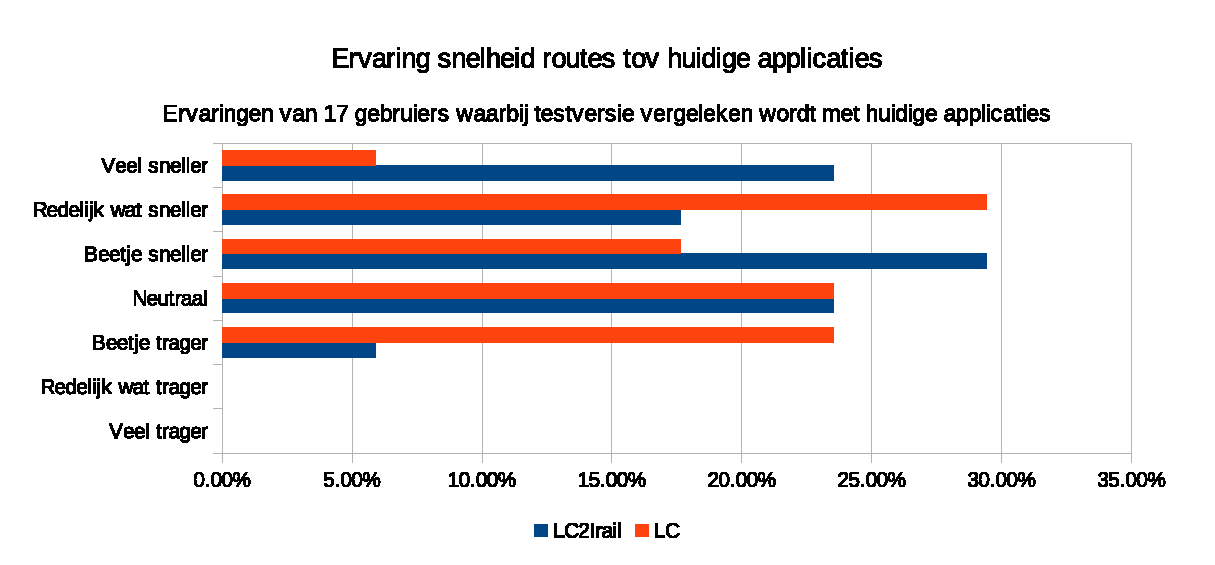
\includegraphics[width=1.00\textwidth]{userdata_routes_currentapp.eps}
	\caption[Door gebruikers ervaren snelheid routes tov huidige apps]{De door 17 gebruikers ervaren snelheid routes ten opzichte huidige apps }
	\label{fig:relativePerceptionRoutes}
\end{figure}

Als tot slot gevraagd wordt om de snelheid te vergelijken met de applicatie die de gebruiker op dit moment gebruikt, doen beide testversies het goed ten opzichte van de huidige applicaties. Dit is zichtbaar in figuur \ref{fig:relativePerceptionRoutes}. Linked Connections scoort iets minder goed dan LC2Irail, maar de overgrote meerderheid vindt Linked Connections nog steeds even snel of sneller dan de applicatie die men gewoonlijk gebruikt.

\section{Voertuigen}

\subsection{Metingen}
Het opzoeken van het traject dat een voertuig aflegt heeft als groot verschil dat incrementele resultaten niet door de gebruikte applicatie ondersteund worden. De reden hiervoor is dat het traject van het voertuig het enige en volledige resultaat is dat de gebruiker wenst, in tegenstelling tot liveboards en routes, waar de gebruiker niet het volledige, maar slechts een deel van het resultaat wenst te zien. 

Dit is ook de opzoeking die het meeste data vereist bij Linked Connections: alle pagina's moeten doorzocht worden op connecties met betrekking tot één specifiek voertuig. Dit voertuig komt slechts in een relatief beperkt aantal pagina's voor, gezien het voertuig slechts enkele uren rijdt, en het tijdstip van eerste vertrek en aankomst onbekend zijn. Zoals eerder vermeld %TODO: referntie
zijn hier enkele oplossingen voor, zoals het gebruik van een index. We definiëren een index in deze context als een lijst van alle treinen voor een bepaalde periode (in dit geval mei 2018) en het tijdstip van hun eerste vertrek.

Om een idee te krijgen van de invloed van deze index, alsook van het gebruik van een cachegeheugen voor de Linked Connections pagina's bij deze opzoekingen, werden 102 voertuigen opgezocht, voor alle combinaties van cache en index gebruik. Tevens werd een extra test gedaan met een cache die in het RAM geheugen geplaatst wordt (in tegenstelling tot het flashgeheugen van het toestel), en een vergelijkende test waarbij de Linked Connections server gebruikt werd. De gemiddelde opzoektijd hiervoor is gevisualiseerd in figuur \ref{fig:vehiclelabtest}.

\begin{figure}[h]
	\centering
	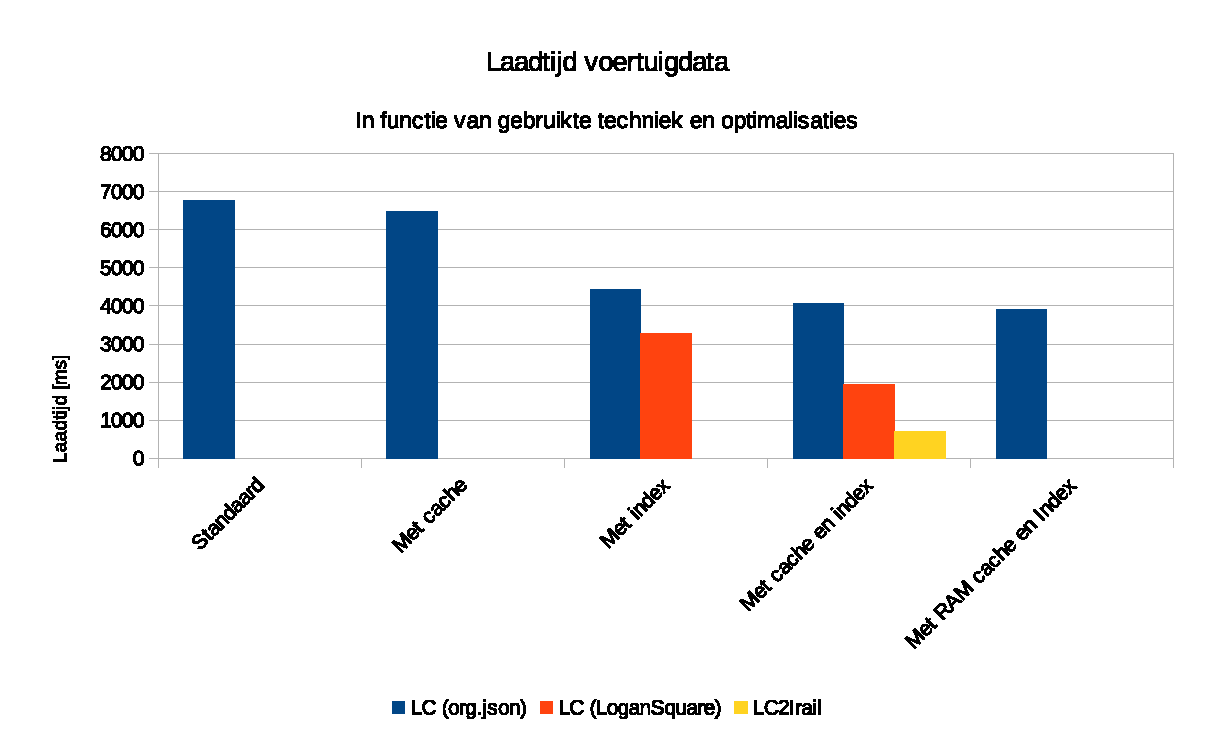
\includegraphics[width=1.00\textwidth]{Optimalisaties_voertuigen.eps}
	\caption[Gemeten laadtijd voertuigen]{De gemeten laadtijd voor voertuigen gebruikmakend van een HTC 10 voor 102 opzoekingen gebaseerd op de iRail logs. }
	\label{fig:vehiclelabtest}
\end{figure}

%\begin{table}[ht]
%	\begin{tabular}{| c | c | c | c | c | c | c |}
%		\hline
%		Variant & parser & cache & index & minimaal (ms) & gemiddelde (ms) & maximaal (ms)\\
%		\hline
%		LC op toestel & org.json & nee & nee & 540 & 6764 & 12676 \\
%		LC op toestel & org.json & ja & nee & 483 & 6488 & 10921 \\
%		
%		LC op toestel & org.json & nee & ja & 2638 & 4443 & 10956 \\
%		LC op toestel & org.json & ja & ja &  2440 & 4066 & 6003\\
%		LC op toestel & org.json & RAM & ja & 2263 & 3912 & 5763 \\
%		LC op toestel & LoganSquare & nee & ja &  1860 & 3283 & 5374 \\
%		LC op toestel & LoganSquare & ja  & ja & 1195 & 1925 & 2888 \\
%		
%		LC op server &&&&  264 & 713 & 5068 \\
%		\hline
%	\end{tabular}
%	\caption[Gemeten laadtijd voertuigen]{De gemeten laadtijd voor voertuigen gebruikmakend van een HTC 10 voor 102 opzoekingen gebaseerd op de iRail logs. }
%	\label{tab:vehiclelabtest}
%\end{table}

Het is duidelijk dat de standaard implementatie zeer slecht presteert. Ook het gebruik van een cachegeheugen brengt hierbij niet veel beterschap. Wanneer echter een index toegevoegd worden, is een drastische verbetering merkbaar. Het gemiddelde daalt in deze beeperkte test met ongeveer een derde. Toevoeging van een cachegeheugen, op flash of in het RAM geheugen, brengt ook hier slechts weinig beterschap. 

Een tweede grote verbetering kan behaald worden door het gebruik van de eerder besproken LoganSquare parser. Hierbij zien we ook een veel grotere verbetering door cachegebruik dan bij de org.json parser. Dit is logisch, gezien bij het gebruik van de LoganSquare parser het verwerken van de data relatief gezien minder tijd in beslag neemt - het ophalen van data wordt dus belangrijker. Op het eerste zicht blijven alle lokale varianten veel trager dan de serverimplementatie, die sneller door pagina's kan zoeken.

We onderzoeken nu het verschil tussen de lokale implementatie en de serverimplementatie in detail. Hiervoor zoeken we 1620 voertuigen op die plaatsvinden op 6 mei 2018. Dit wordt enerzijds gedaan voor de lokale implementatie die gebruik maakt van de LoganSquare parser, cache en lokale index, en anderzijds voor de serverimplementatie, die server-side over dezelfde index en een cache beschikt.

Wanneer we kijken naar de box-plot van de responstijd, weergegeven in figuur \ref{fig:vehicleboxplot}, zien we dat de lokale implementatie duidelijk slechter presteert. Op beide toestellen is LC2Irail sneller dan Linked Connections. Bij de HTC 10, een snel toestel, valt dit nog enigszins mee, maar op de HTC One zijn de meeste resultaten binnen 3000 milliseconden geladen, terwijl op dat moment nog geen 25\% van de opzoekingen via Linked Connections uitgevoerd werd. Ook zien we hier dat LC2Irail consistente prestaties biedt: beide box plots zijn praktisch identiek, op wat uitlopers na. Voor Linked Connections zien we echter dat, net zoals voor het opzoeken van liveboards en routes, de spreiding van de benodigde tijd afhangt van het toestel: een traag toestel heeft een grotere variatie in de laadtijd.

\begin{figure}[h]
	\centering
	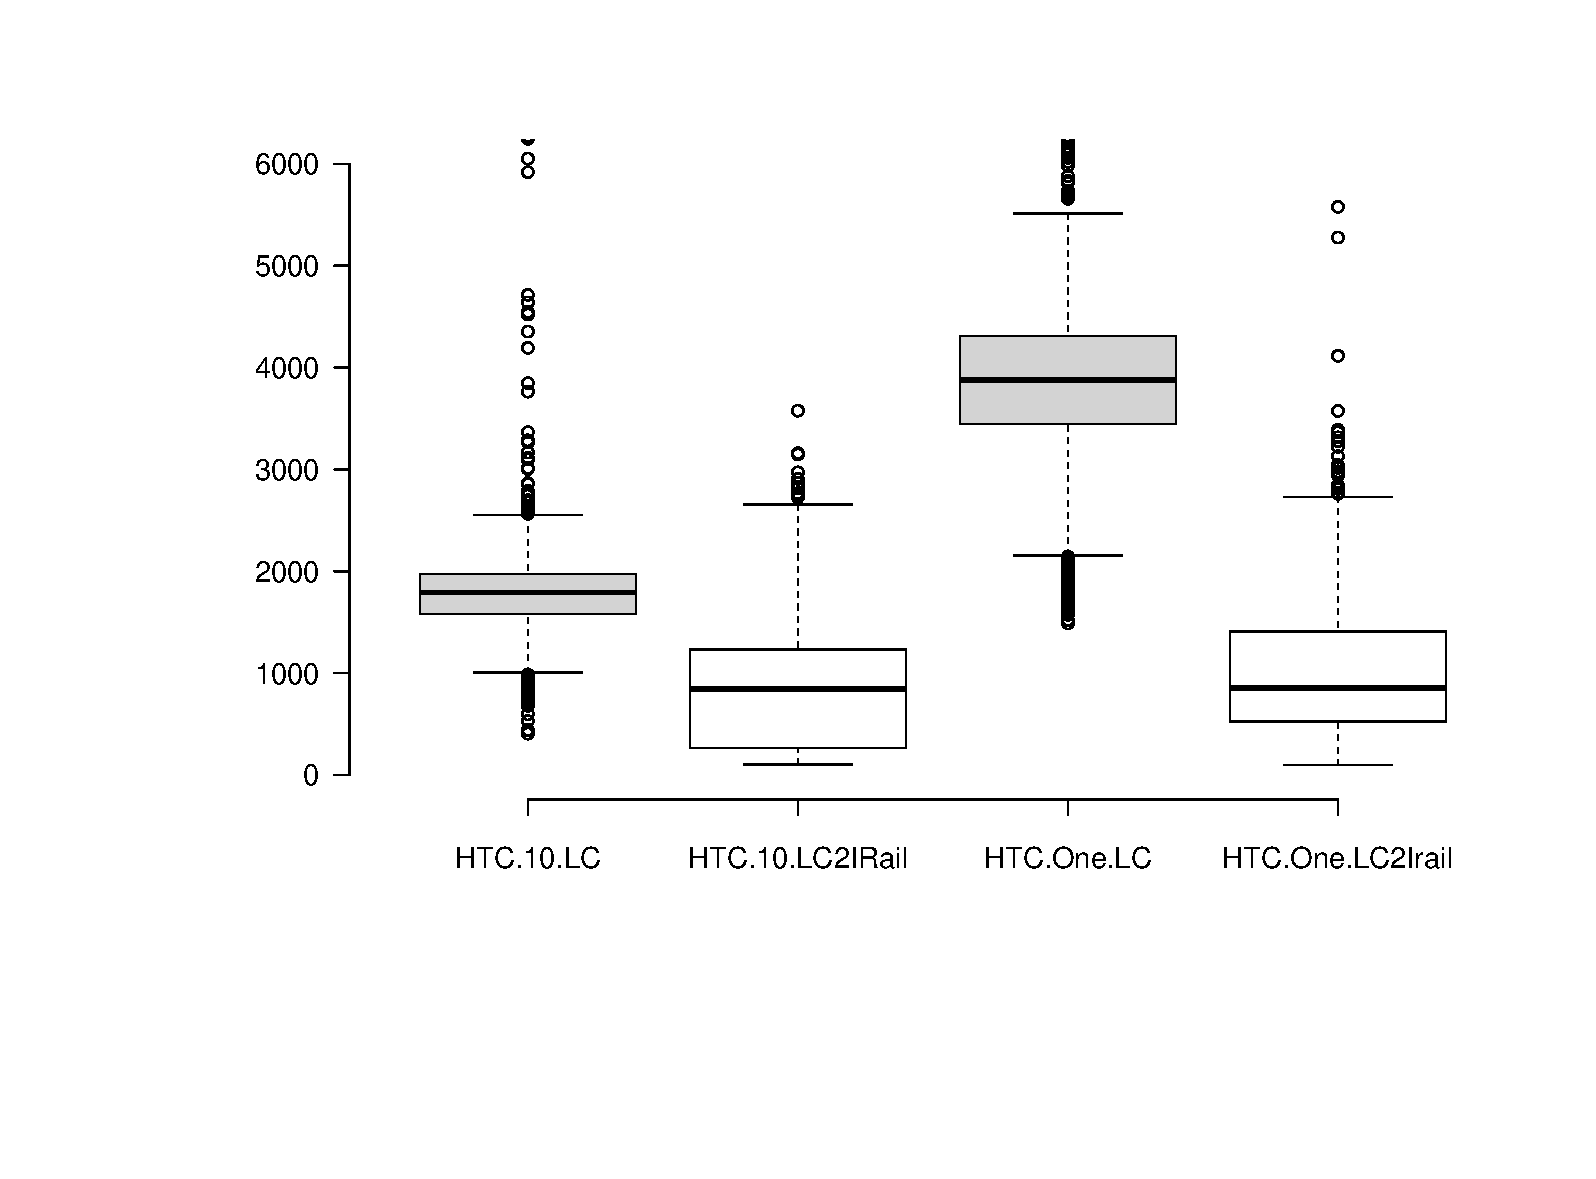
\includegraphics[width=1.00\textwidth]{boxplot_vehicles.eps}
	\caption[Prestaties voor het laden van voertuigen]{De prestaties voor het laden van voertuigen, gemeten door alle voertuigen, beschreven in Linked Connections, voor 6 mei op te zoeken.}
	\label{fig:vehicleboxplot}
\end{figure}

%\begin{figure}[h]
%	\centering
%	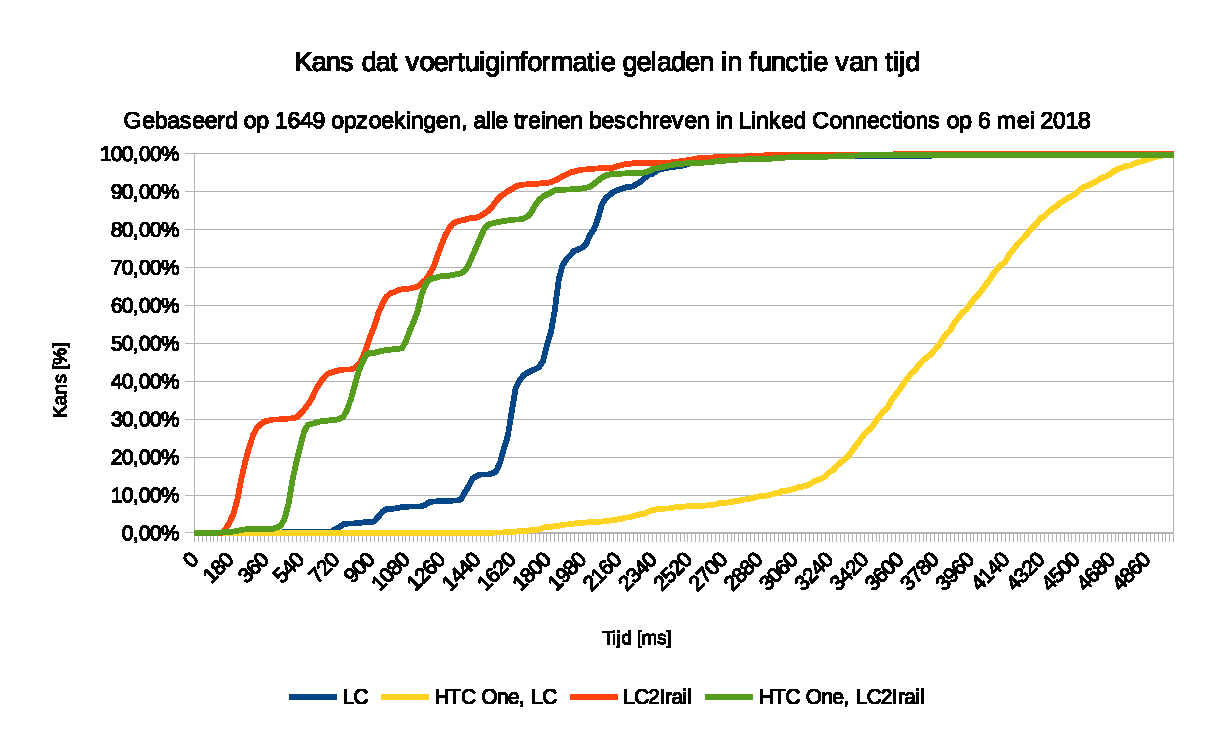
\includegraphics[width=1.00\textwidth]{distribution_vehicle_loading_cummulatief.eps}
%	\caption[Cummulatieve kans op laden van voertuig]{De kans dat een voertuig geladen is in functie van de verlopen tijd.}
%	\label{fig:vehiclecummulatief}
%\end{figure}

\subsection{Ervaringen}
Wanneer we nu de resultaten van de user-testing bekijken, zien we zoals verwacht dat het laden van voertuigen beduidend slechter scoort wanneer de lokale Linked Connections implementatie gebruikt wordt, vergeleken met wanneer de serverimplementatie gebruikt werd. In figuur \ref{fig:vehicleboxplot} is dit duidelijk zichtbaar. Zo beoordelen de meeste gebruikers Linked connections slechts als "gemiddeld", terwijl de meerderheid van de gebruikers de LC2Irail variant als "Zeer snel" bestempelde. Ook zien we hier, net als bij liveboards en routes, dat er voor Linked Connections een veel grotere spreiding is in de gegeven antwoorden, terwijl  bij LC2Irail iedereen het er over eens lijkt dat deze implementatie snel is.

\begin{figure}[h]
	\centering
	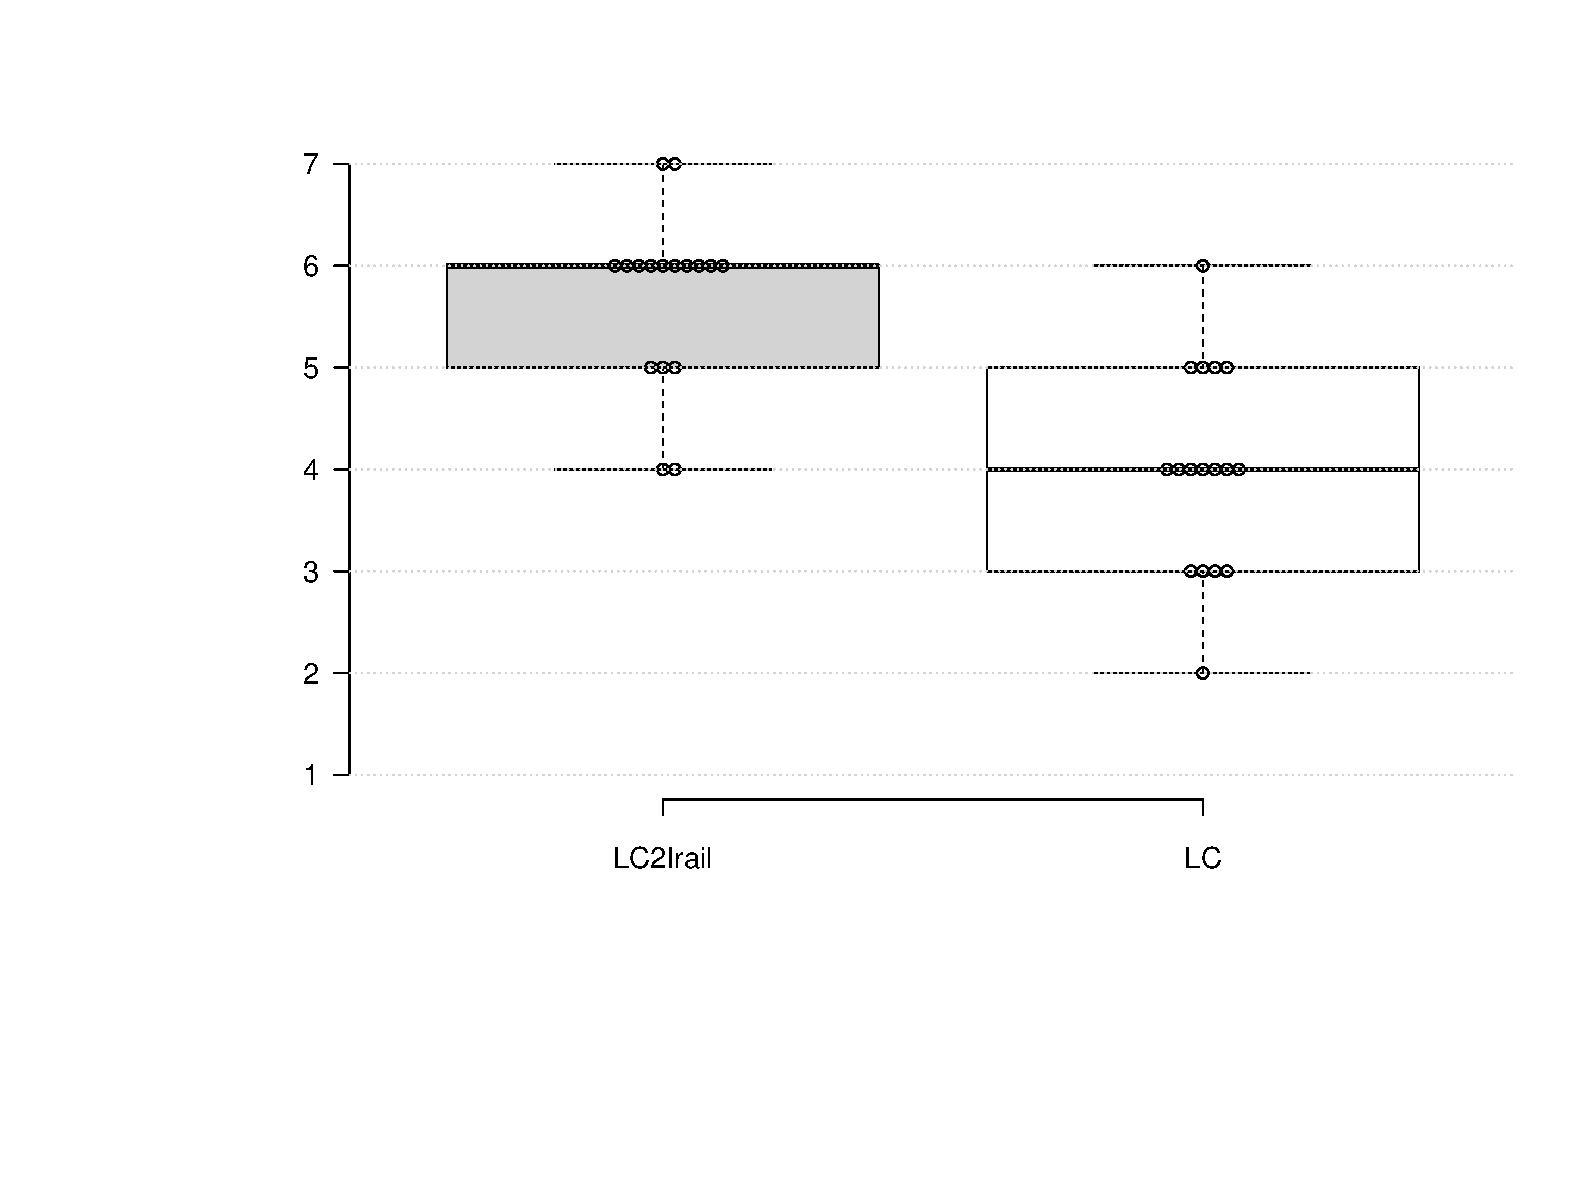
\includegraphics[width=1.00\textwidth]{boxplot_vehicles_ux.eps}
	\caption[Ervaren snelheid van routes]{De ervaren snelheid op een schaal 1-7 van routes voor LC2Irail en Linked Connections, gebaseerd op 17 user tests.}
	\label{fig:vehiclesUx}
\end{figure}

Personen die de lokale implementatie op basis van \foreign{LoganSquare} testten, beoordeelden de laadtijd iets beter vergeleken met de groep die de implementatie op basis van de \foreign{org.json} parser testte. Ondanks dat de testgroep onvoldoende groot was om een veralgemening te kunnen maken, kunnen we wel stellen dat er een grote kans is dat verbeteringen in de implementatie de snelheid verder omlaag kunnen brengen, en zo de gebruikerservaring kunnen verbeteren. Gezien bij het berekenen van voertuigen het meeste data nodig is, is hier de impact van implementatiedetails het grootst.

\begin{figure}[ht]
	\centering
	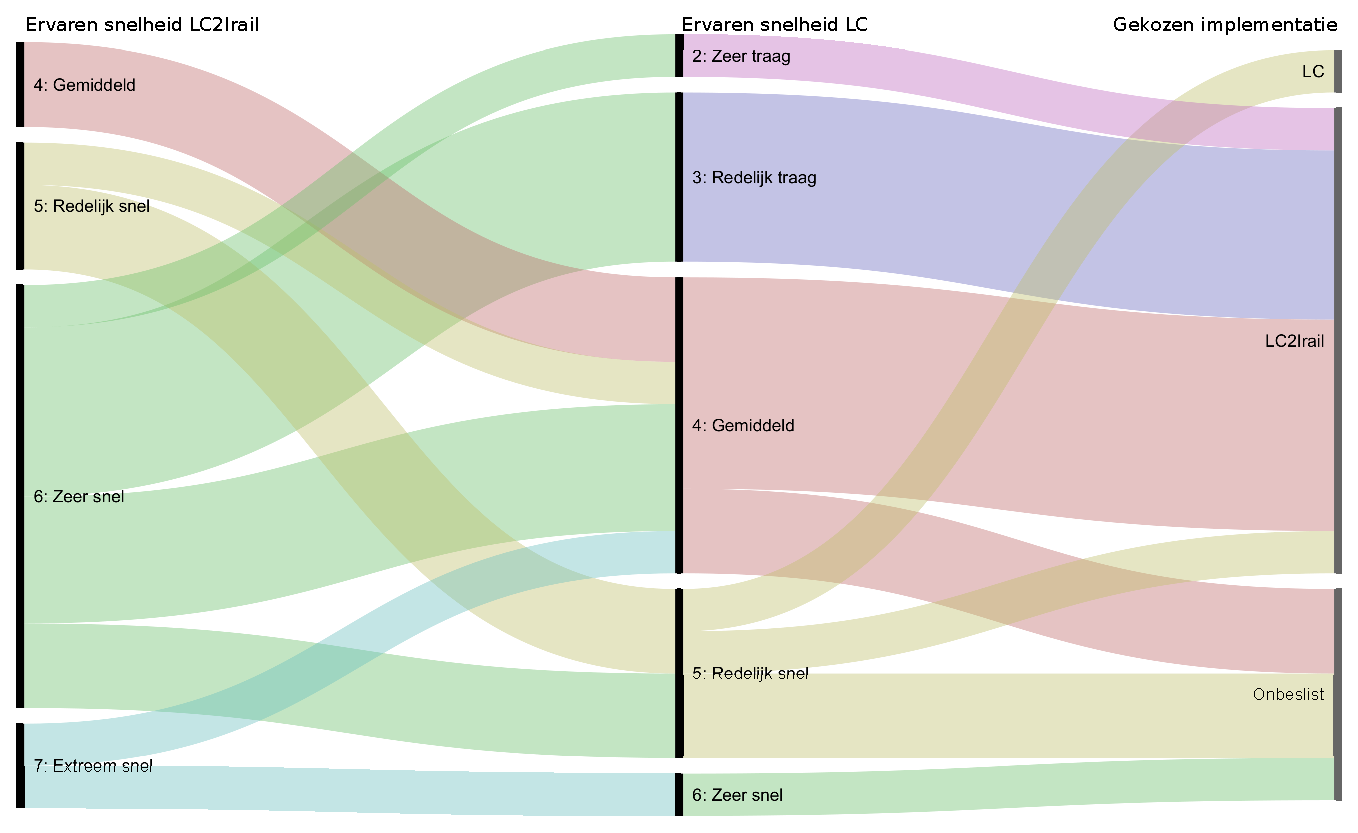
\includegraphics[width=1.00\textwidth]{alluvial_user_choice_vehicles.eps}
	\caption[Door gebruikers gekozen implementatie voor voertuigen]{Verbanden tussen de door gebruikers gekozen implementaties voor voertuigen. }
	\label{fig:alluvialUserChoicesVehicles}
\end{figure}

Wanneer de gebruiker gevraagd werd te kiezen, koos slechts één gebruiker voor de lokale implementatie in dit onderdeel. Vijf gebruikers hadden geen specifieke voorkeur voor een specifieke implementatie, ook al beoordeelden vier van hen Linked Connections als trager. In figuur \ref{fig:alluvialUserChoicesVehicles} zijn de ervaringen van elke gebruiker duidelijk te zien. Zo zien we dat de ervaring voor gebruikers nooit verbeterd, en veel gebruikers een groot verschil ervaren tussen de snelheid van beide implementaties, in het nadeel van Linked Connections. Veel gebruikers die Linked Connections als redelijk of zeer snel ervaren, ervoeren LC2Irail nog steeds als sneller, waardoor ze wanneer ze moesten kiezen niet voor Linked Connections kozen. De enigste gebruiker die voor Linked Connections koos, ervoer Linked Connections niet als sneller dan LC2Irail, maar vond beide wel snel.

Als gevraagd wordt om de snelheid te vergelijken met de applicatie die de gebruiker op dit moment gebruikt, geven zes op tien gebruikers aan Linked Connections als even snel te ervaren voor het opzoeken van voertuigen, en telkens één op tien gebruikers ervaart LC als een beetje trager, een beetje sneller of veel sneller. Net zoals bij het opzoeken van routes ervaart de helft van de testers LC2Irail als even snel om voertuigen op te zoeken, telkens een zesde ervaart LC2Irail als een beetje, redelijk of veel sneller dan de app die men gewoonlijk gebruikt.

Uit de combinatie van metingen en ervaringen concluderen we dat gebruikers de laadtijd van voertuigdata acceptabel tot snel vinden voor Linked Connections. Een seconde of meer langer laden, wat vaak geval is bij Linked Connections, zorgt bij veel mensen voor een slechtere ervaring. De impact hiervan wordt verder besproken in hoofdstuk \ref{chap:interpretatie}.

\section{Door de gebruiker gekozen implementatie}

Voor alle soorten informatie (liveboards, routes, en voertuigen) lijkt Linked Connections een slechtere gebruikerservaring dan LC2Irail, in termen van laadtijd. Hierbij dienen we op te merken dat dit verschil bij liveboards slechts zeer beperkt is, en het laden nog steeds als snel werd ervaren. Voor routes bestempelden enkele personen Linked Connections als traag, maar blijft het verschil beperkt. Bij voertuigen blijkt echter dat Linked Connections door drie kwart van de gebruikers als trager werd ervaren, waarbij Linked Connections niet enkel relatief slechter scoort, maar ook in absolute termen slechts door een minderheid van de gebruikers als snel wordt ervaren. 

Dit zien we ook terug in de antwoorden wanneer gebruikers gevraagd werd te kiezen tussen beide implementaties. Voor vertrekken zijn er vier gebruikers die beide implementaties even snel vinden, terwijl van de overige 13 slechts vijf kiezen voor Linked Connections. Bij routes en voertuigen scoort Linked Connections zoals verwacht slechter: er zijn respectievelijk slechts twee en een gebruiker die voor Linked Connections kiezen zijn. Hierbij zijn er respectievelijk twee en vijf gebruikers die geen verschil tussen de implementaties merkten. De keuzes van gebruikers werden uitgezet in figuur \ref{fig:alluvialUserChoices}. In dit diagram zien we zowel hoeveel gebruikers voor elke implementatie kozen, maar ook hoe de keuze van gebruiker evolueert. Zo zien we dat naarmate de relatieve prestaties van LC ten opzichte van LC2Irail dalen, personen die eerder voor Linked Connections kozen overstappen op LC2Irail.

\begin{figure}[ht]
	\centering
	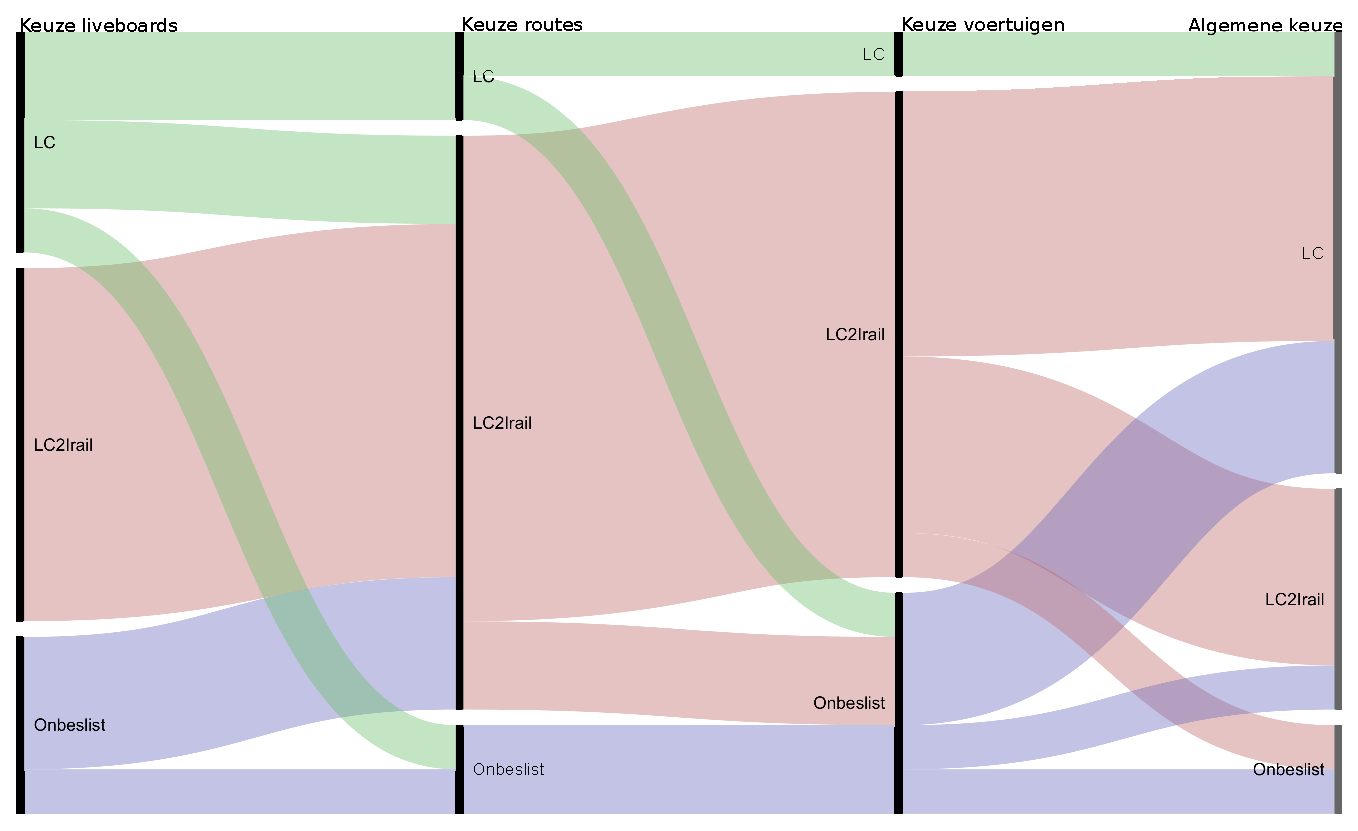
\includegraphics[width=1.00\textwidth]{alluvial_user_choice.eps}
	\caption[Door gebruikers gekozen implementatie]{Verbanden tussen de door gebruikers gekozen implementaties voor alle soorten informatie, alsook de resulterende keuze waarbij ook offline toegang in rekening werd gebracht. }
	\label{fig:alluvialUserChoices}
\end{figure}

Terwijl de meerderheid van de gebruikers steeds voor LC2Irail koos, kantelt deze balans echter volledig om wanneer gebruikers worden gevraagd om met alle aspecten rekening te houden. Dit is duidelijk zichtbaar aan de rechterkant van figuur \ref{fig:alluvialUserChoices}. Hieruit blijkt duidelijk dat gebruikers enige snelheid willen opgeven in ruil voor offline opzoekingen. Zeven gebruikers laten weten dat ze een hybride systeem ideaal zou zijn, waarbij de snelheid van LC2Irail gecombineerd wordt met Linked Connections als offline alternatief. Wanneer deze gebruikers alsnog verplicht werden te kiezen, waren hun keuzes gelijk verdeeld, afhankelijk van de persoonlijke nood om offline te kunnen opzoeken. 


We trachten nu een antwoord te vinden op de in hoofdstuk \ref{chap:onderzoek} gestelde vragen.
\begin{itemize}
	\item Ervaart de gebruiker een app die lokaal Linked Connections gebruikt als sneller dan een app die gebruik maakt van een RPC API?\\
	De ervaring van de gebuiker hangt sterk af van het gebruikte toestel en de gemaakte opzoekingen. Enkel gebruikers van snelle toestellen ervaren Linked Connections in sommige gevallen als sneller. Voor liveboards is Linked Connections concurrentieel, maar voor andere opzoekingen is deze techniek meestal trager dan de gebruikte RPC API.
	\item Ervaart de gebruiker een app die lokaal Linked Connections gebruikt als sneller dan zijn huidige app?\\
	Een minderheid ervaart Linked Connections als sneller dan de huidige gebruikte applicatie. Voor liveboards, routes en voertuigen vinden respectievelijk 45\%, 30\% en 24\% dat Linked Connections sneller is. Respectievelijk 30\%, 40\% en 60\% van de gebruikers ervaren Linked Connections als even snel, met 24\%, 30\% en 12\% van de gebruikers die Linked Connections expliciet als trager ervaren dan hun huidige applicatie. Linked Connections brengt op dit moment zeker geen verbetering in snelheid voor de gebruikers.
\end{itemize}

Wat dit wilt zeggen voor de onderzoeksvraag en hypotheses en zullen we verder bespreken in hoofdstuk \ref{chap:interpretatie}.

\section{Enquete}
Zoals vermeld in hoofdstuk \ref{chap:onderzoek}, trachten we een aantal vragen te beantwoorden aan de hand van een enquete (bijlage \ref{appendix:enquete}). We zullen nu eerst de resultaten van deze enquete overlopen, alvorens aan de hand van deze resultaten een antwoord te formuleren op de in hoofstuk \ref{chap:onderzoek} geformuleerde vragen.

\subsection{Antwoorden van respondenten}
Er werden in totaal 81 volledig ingevulde enquetes digitaal verzameld, in een gevarieerd publiek. Zo neemt meer dan de helft van de respondenten meerdere keren per week (26\%) of dagelijks (28\%) de trein. Ook personen die occasioneel reizen zijn goed vertegenwoordigt, zo reist 16\% minder dan één keer per maand per trein.

Wanneer we kijken naar de informatiebronnen voor reizigers, blijkt dat \foreign{native} applicaties voorop staan (93\%, waarvan 27\% third-party applicaties zijn), gevolgd door digitale informatieborden en affiches (74\%) en websites (62\%) . Hierbij moeten we opmerken dat de enquete specifiek gericht is op personen die applicaties gebruiken om informatie op te zoeken, en het werkelijk aandeel van de reizigers die applicaties gebruikt dus iets lager kan liggen.

Iets minder dan de helft (48\%) van de treinreizen verloopt probleemloos. Alle respondenten geven aan vertragingen te ervaren bij het reizen, waarbij 33\% aangeeft meestal of altijd vertraging te hebben. Na vertragingen zijn spoorwijzigingen de tweede grootste bron van ergernis: meer dan 85\% van de gebruikers ervaart dit wel eens, waarbij dit voor 15\% van de reizigers regelmatig voorvalt. Tot slot geeft 72\% van de respondenten aan wel eens een afgeschafte trein te hebben, al gebeurt dit voor amper 1\% de helft van de tijd.

Wanneer we kijken naar hoe up-to-date informatie voor reizigers is, wordt duidelijk dat hier zeker ruimte is voor verbetering: slechts 25\% zegt altijd over actuele informatie in de stations te beschikken, applicaties doen het iets beter, waarbij 40\% van de gebruikers altijd over actuele informatie beschikt. Voor beide blijkt dat 50\% van de personen die dit ervaart, er slechts soms last van heeft. Echter blijkt wel dat 27\% van de personen minstens de helt van de tijd dit probleem in stations ervaart. Applicaties doen het iets beter, waar slechts 10\% van de gebruikers dit probleem minstens de helft van de tijd ervaart. Uit deze cijfers kunnen we concluderen dat gebruikers wel degelijk nood hebben aan actuele informatie. 

Applicaties blijken ook de voornaamste bron van informatie te zijn voor gebruikers: Voor alle problemen, op spoorwijzigingen na, checken gebruikers hun smartphone. Voor spoorwijzigingen blijft informatie in de stations zelf, zoals omgeroepen informatie of digitale borden populairder. Ook wanneer informatie in de applicatie niet actueel is zoeken mensen hun toevlucht tot de omgeroepen informatie of digitale borden. Wanneer gebruikers gevraagd worden om informatiebronnen naar gebruik te rangschikken, blijven applicaties en websites ook hier bovenaan staan.

Wanneer we nu gaan kijken naar de tevredenheid, blijkt dat applicaties hier uitzonderlijk goed scoren: meer dan 77\% van de gebruikers is hierover tevreden. Dit vormt een scherp contrast met websites, waar slechts 43\% tevreden over is. Voor alle informatiebronnen zijn er ontevreden gebruikers, wat er opnieuw op wijst dat er ruimte is voor verbetering.

Bij de respondenten zijn Android en iOS gelijk vertegenwoordigd, met respectievelijk 39 en 40 respondenten. Een enkele respondent gebruikt Windows Mobile, nog een enkeling gebruikt Sailfish OS. 73\% gebruikt voornamelijk de officiele NMBS applicatie, de andere 27\% is ongeveer gelijk verdeeld over third-party applicaties, zoals HyperRail, iRail, Railer en BeTrains (tesamen goed voor 21\%) en een mix van algemene en buitenlandse applicaties, zoals citymapper, de Lijn en Deutsche Bahn.

Deze applicaties gebruiken we vooral in stations (95\% van de gebruikers), maar ook thuis (85\%) en op de trein zelf (80\%). Op de trein zijn we echter niet tevreden over de snelheid waarmee resultaten laden (66\% tevreden), thuis zijn we iets tevredener (72\% tevreden). Ook de gebruiksvriendelijkheid van opzoekingen daalt tijdens het reizen. 

Naar mogelijke oorzaken van deze dalingen tijdens een reis hoeven we niet ver te zoeken: 60\% van de reizigers is ontevreden over het mobiele netwerk tijdens een treinreis. Maar liefst 96\% van de reizigers heeft last van traag of niet ladende webpagina's, de meerderheid van hun ondervind hier minstens de helft van de tijd hinder door. Diezelfde mobiele data is voor 53\% van de respondenten ook een bron van angst - ondanks dat er steeds meer data bij abonnementen geleverd wordt, blijven we schrik hebben om te veel data te verbruiken. Hier dienen we wel onmiddellijk te nuanceren: 21\% maakt zich slechts een beetje zorgen. Deze groep zal vermoedelijk vooral voorzichtig zijn met media, en niet zozeer met het gebruik van routeplanning applicaties. Vooral jongeren (jonger dan 18) en personen ouder dan 35 jaar zijn voorzichtig met hun mobiele data.

Wanneer we informatie niet opzoeken via de app, is dit voornamelijk omdat de gebruiker geen mobiele data heeft (33\%), omdat het opzoeken te lang doet (24\%), of omdat informatie in het station handiger is. We maken ons iets meer zorgen om het batterijverbruik van de applicatie (19\%) dan om het dataverbruik (15\%).

Wanneer gebruikers gevraagd wordt naar wat ze belangrijk vinden in een applicatie voor openbaar vervoer, komt het snel laden van resultaten overduidelijk op de eerste plaats. Dit wordt gevolgd door offline zoekopdrachten, waarna privacy, batterijverbruik en dataverbruik kort op elkaar volgen.

Ondanks dat privacy een hot topic is, geeft 53\% van de gebruikers aan zich hier geen zorgen om te maken. Dit zouden we misschien beter wel doen, want 75\% weet niet zeker of zijn of haar reisplannen over internet verstuurd worden, terwijl alle applicaties dit op dit moment doen. 12\% is er zelfs zeker van overtuigd dat zijn of haar reisplannen niet over internet verzonden worden. Ook over het versturen van onze locatie zijn we slecht geïnformeerd. Zo meent 17\% onterecht dat zijn of haar exacte locatie waarschijnlijk niet over internet verstuurd wordt. Voor third-party apps waarvan we zeker weten dat ze de locatie niet over internet versturen, blijkt dan weer dat verschillende personen onterecht denken dat hun locatiegegevens toch verstuurd worden. 

Terwijl de meerderheid aangaf niet wakker te liggen van hun privacy bij routeplanning applicaties, blijkt toch dat het 85 en 77 percent van de respondenten zou storen moesten respectievelijk hun locatie en reisplannen over internet verstuurd worden.
 
Overstappen naar een andere applicatie is voor velen echter een brug te ver: slechts 35 en 37 percent van de respondenten zou overstappen naar een applicatie die respectievelijk hun reisplannen en locatie niet over internet verstuurd. Een ongeveer even groot aandeel geeft aan dat ze dit misschien zouden doen, afhankelijk van wat de alternatieven zijn. Deze aantallen dienen we ook onmiddelijk te nuanceren: ondanks recente privacyschandalen, blijft het overgrote deel van de smartphonegebruikers messaging apps als Facebook Messenger en Whatsapp gebruiken, ondanks de beschikbaarheid van veiligere en privacyvriendelijkere applicaties. Overstappen en wennen aan een nieuwe applicatie kost moeite en tijd, wat veel gebruikers er niet voor over hebben.

Tot slot werden gebruikers bevraagd naar wat ze vinden van een applicatie op basis van Linked Connections. Twee personen gaven aan de uitleg niet volledig te begrijpen, en zijn van deze analyse uitgesloten.
Respondenten werden gevraagd om de vier voornaamste voordelen van Linked Connections voor gebruikers van meest naar minst belangrijk te ordenen. Ondanks dat de gebruikers geïnformeerd werden dat Linked Connections volledige privacy biedt, en dat ongeveer een derde aan gaf over te stappen naar een privacyvriendelijke applicatie, komt privacy slechts bij 15\% op de eerste plaats, en bij meer dan de helft zelfs op de vierde plaats. Snelheid blijft koploper, gevolgd door offline zoeken, aangepaste routes en tot slot privacy.

Dat aangepassen van routeplanning en privacy slechts op de vierde plaats komen wilt niet zeggen dat men dit niet belangrijk vindt. Tijdens user tests gaven testers reeds aan deze rangschikkingen moeilijk te vinden, en wanneer gepolst wordt naar de interesse in afzonderlijke aspecten, blijkt dat mensen vooral het aanpassen van routeplanning en offline zoeken enorm interessant vinden, gevolgd door snelheid en privacy. Bij het aanpassen van routeplanning willen reizigers vooral kunnen zoeken naar routes met een kortere overstaptijd, drukke treinen mijden, en routes plannen met wat meer tijd om over te stappen. Privacy, wat op de laatste plaats staat, blijft interessant voor 83\% van de respondenten. Hieruit kunnen we besluiten dat Linked Connections enorm veel potentieel heeft voor mobiele applicaties. We zullen deze resultaten nog verder bespreken in hoofstud \ref{chap:interpretatie}.
\subsection{Conclusies op basis van de enquete}
We zullen nu een antwoord formuleren op de in hoofdstuk \ref{chap:onderzoek} geformuleerde vragen.
\begin{itemize}
	\item Bied offline informatie een meerwaarde voor gebruikers?\\
	Ja, gebruikers hebben grote interesse in offline opzoekingen, voornamelijk door een slechte mobiele internetverbinding tijdens het reizen, en in mindere mate omdat ze vrezen te veel data te verbruiken of gewoonweg niet over mobiel internet beschikken.
	\item Hecht de gebruiker belang aan privacy bij het gebruik van routeplanning apps? Zo ja, in welke mate?\\
	De gebruiker hecht in beperkte mate belang aan zijn of haar privacy bij gebruik van routeplanning apps. De helft zegt zich hier geen zorgen over te maken, maar slechts een minderheid van de gebruikers weet welke data over internet verzonden wordt. Een derde van de gebruikers zou overstappen naar apps die privacyvriendelijker zijn.
	\item Heeft de gebruiker schrik om te veel mobiele data te verbruiken?\\
	Ongeveer de helft van de gebruikers heeft schrik om te veel mobiele data te gebruiken, al maakt slechts een derde van de gebruikers zich hier ernstig zorgen om.
	\item Hecht de gebruiker belang aan dataverbruik bij het gebruik van routeplanning apps?\\
	Één op zes gebruikers geeft aan soms geen informatie met een applicatie op te zoeken uit vrees te veel data te verbruiken. Wanneer gebruikers echter gevraagd wordt om een aantal aspecten van een routeplanning applicatie van belangrijk naar onbelangrijk te rangschikken, eindigt dataverbruik op de laatste plaats. Dataverbruik is voor de gebruiker dus van ondergeschikt belang aan de functionaliteit.
	\item Is de gebruiker tevreden met de snelheid van zijn huidige routeplanning app?\\
	Thuis zijn zeven op tien gebruikers tevreden met de snelheid van routeplanning applicaties. Onderweg daalt dit tot een derde, hoogstwaarschijnlijk door slechte netwerkverbindingen.
	\item Wat is voor een gebruiker belangrijk in routeplanning apps?\\
	Gebruikers vinden vooral het snel laden van resultaten belangrijk. Na snelheid volgen offline zoekopdrachten, waarna privacy, batterijverbruik en dataverbruik ongeveer even belangrijk zijn.
	\item Is de gebruiker geïnteresseerd in routeplanning op maat? Zo ja, welke aspecten spreken hem dan aan?\\
	De gebruiker is zeer geïnteresseerd in routeplanning op maat, waarbij vooral het aanpassen van de overstaptijd in stations belangrijk is, en ook het mijden van drukke treinen als zeer interessant beschouwd wordt.
	\item Is de gebruiker geïnteresseerd in offline opzoekingen?\\
	Zoals eerder vermeld vormen offline opzoekingen een meerwaarde voor gebruikers. Wanneer expliciet bevraagd, blijkt dan ook dat veel gebruikers hier in grote mate in geïnteresseerd zijn.
	\item Is de gebruiker geïnteresseerd in de mogelijke snelheid die Linked Connections biedt?\\
	Ondanks dat veel gebruikers al tevreden zijn met de huidige snelheid van routeplanning applicaties, blijft het overgrote deel geïnteresseerd in het verder versnellen van deze applicaties.
	\item Is de gebruiker geïnteresseerd in de volledige privacy die Linked Connections biedt?\\
	Ondanks dat privacy steevast onderaan de lijst met prioriteiten van gebruikers staat, wilt dit niet zeggen dat gebruikers hierin niet geïnteresseerd zijn. Meer dan acht op tien gebruikers vindt dit interessant.
\end{itemize}

\section{Beperkingen}
\label{sec:beperkingen}
\subsection{Kleine steekproef voor user-testing}
Zoals eerder vermeld ontbreekt op het moment van schrijven nog cruciale informatie in Linked Connections, zoals of een voertuig al dan niet afgeschaft is, en op welk perron een voertuig aankomt. Hierdoor moesten we terugvallen op user-testing onder begeleiding, om gebruikers aan te sporen hun gebruikelijke opzoekingen te doen en te polsen naar hun ervaringen. Dit neemt relatief veel tijd in beslag, waardoor weinig mensen én zin, én tijd hebben. Voorts neemt deze methode van testen ook veel tijd in beslag voor de onderzoeker. 

De groep testgebruikers is wel gevarieerd, zowel in persoonlijke eigenschappen zoals leeftijd, als in reisgewoontes per trein. Wanneer de gehele testgroep duidelijk de voorkeur geeft aan een bepaalde variant, kunnen we deze keuze veralgemenen naar de gehele populatie. Wanneer er echter geen grote meerderheid voor eenzelfde variant kiest, moeten we voorzichtig zijn met conclusies.

\subsection{Beperkt aantal unieke toestellen getest}
Uit de voorgaande secties blijkt dat het gebruikte toestel van groot belang is voor de prestaties van de lokale Linked Connections implementatie. Tijdens het user-testen werd gebruik gemaakt van twaalf verschillende smartphones. Dit aantal is relatief beperkt in vergelijking met het aanbod op de huidige smartphonemarkt. Eventuele verder onderzoek zal de prestaties van Linked Connections op verschillende toestellen moeten vastleggen.

\subsection{Processorverbruik niet meetbaar}
De Android CPU Profiler beïnvloed de prestaties van de applicatie zodanig dat het onmogelijk is om een correct beeld te krijgen van het processorverbruik. Er kan een beeld gevormd worden welke onderdelen van de applicatie het meest processortijd vragen, maar exacte tijdsmetingen zijn niet mogelijk. Deze problemen worden ook door andere Android ontwikkelaars op internet beschreven\footnote{\url{https://stackoverflow.com/questions/49555983/background-concurrent-copying-gc-freed}}. Deze problemen treden op door de nieuwe Android CPU profiler, die zelf teveel processortijd op het apparaat vereist.

\subsection{Prestaties zijn sterk afhankelijk van implementatiedetails}
Zoals blijkt uit grafieken %TODO: REFERENTIE
is de performantie van de lokale Linked Connections implementatie sterk afhankelijk van details in de implementatie - Het is dus niet enkel belangrijk om de algoritmes te optimalizeren, maar ook om rekening te houden met processen zoals Garbage Collection. Dit werd pas in een gevorderd stadium van de proef vastgesteld. Het is mogelijk dat de resultaten in dit onderzoek nog verder verbeterd kunnen worden door dezelfde algoritmes efficiënter te implementeren.